% $Id: Solvers.tex,v 1.2 2008/03/18 16:40:29 dconway Exp $
\chapter{\label{chapter:Solvers}Solvers}
\chapauthor{Darrel J. Conway}{Thinking Systems, Inc.}

\section{Overview}

GMAT implements several algorithms used to tune mission models, so that specific mission goals can
be defined and achieved from within the mission sequence.  The subsystem used for this mission
parameter tuning is the Solver subsystem.

Each of the solvers in GMAT can be described as a finite state machine taking the input state of
the GMAT objects in a mission and changing the states of user specified parameters to achieve
desired goals.  Each solver executes a series of GMAT commands as part of this solution finding
algorithm; the differences between the different solvers comes from the approach taken to find
this solution.

\section{Solver Class Hierarchy}

Each solver takes a section of a mission sequence, and manipulates variables in that subsequence in
order to evaluate how those changes affect the modeled mission.  The results of the changes are
collected in the Solver, reported to the user if desired, and possibly used to drive subsequent
actions in the mission sequence.

The Solver subsystem can be decomposed into three broad categories of algorithms: scanners,
targeters, and optimizers.  The distinguishing characteristics of these different algorithms can be
summarized as follows:

\begin{itemize}
\item \textbf{Scanners} are used to perform studies of the behavior of the the system as the
variables change, in order to collect statistical data about how the system behaves in the
neighborhood of the variables defined for the problem.  A scanner does not have an inherent set of
goals; rather, the intention of a scanner is to evaluate how changes in the system variables affect
the behavior of the system over time.
\item \textbf{Targeters} are used to find solutions that satisfy a set of goals to within some user
defined set of tolerances.  In other words, a targeter is seeking an exact solution, and stops
searching for that solution when the achieved results of the targeter all fall to within a specified
tolerance of those goals.
\item \textbf{Optimizers} are used to find the configuration of the variables that best satisfies a
set of user goals, subject, optionally, to a set of constraints.  Optimizers function by seeking the
minimum of a user defined function of parameters, subject to these constraints.
\end{itemize}

\begin{figure}[tb]
\begin{center}
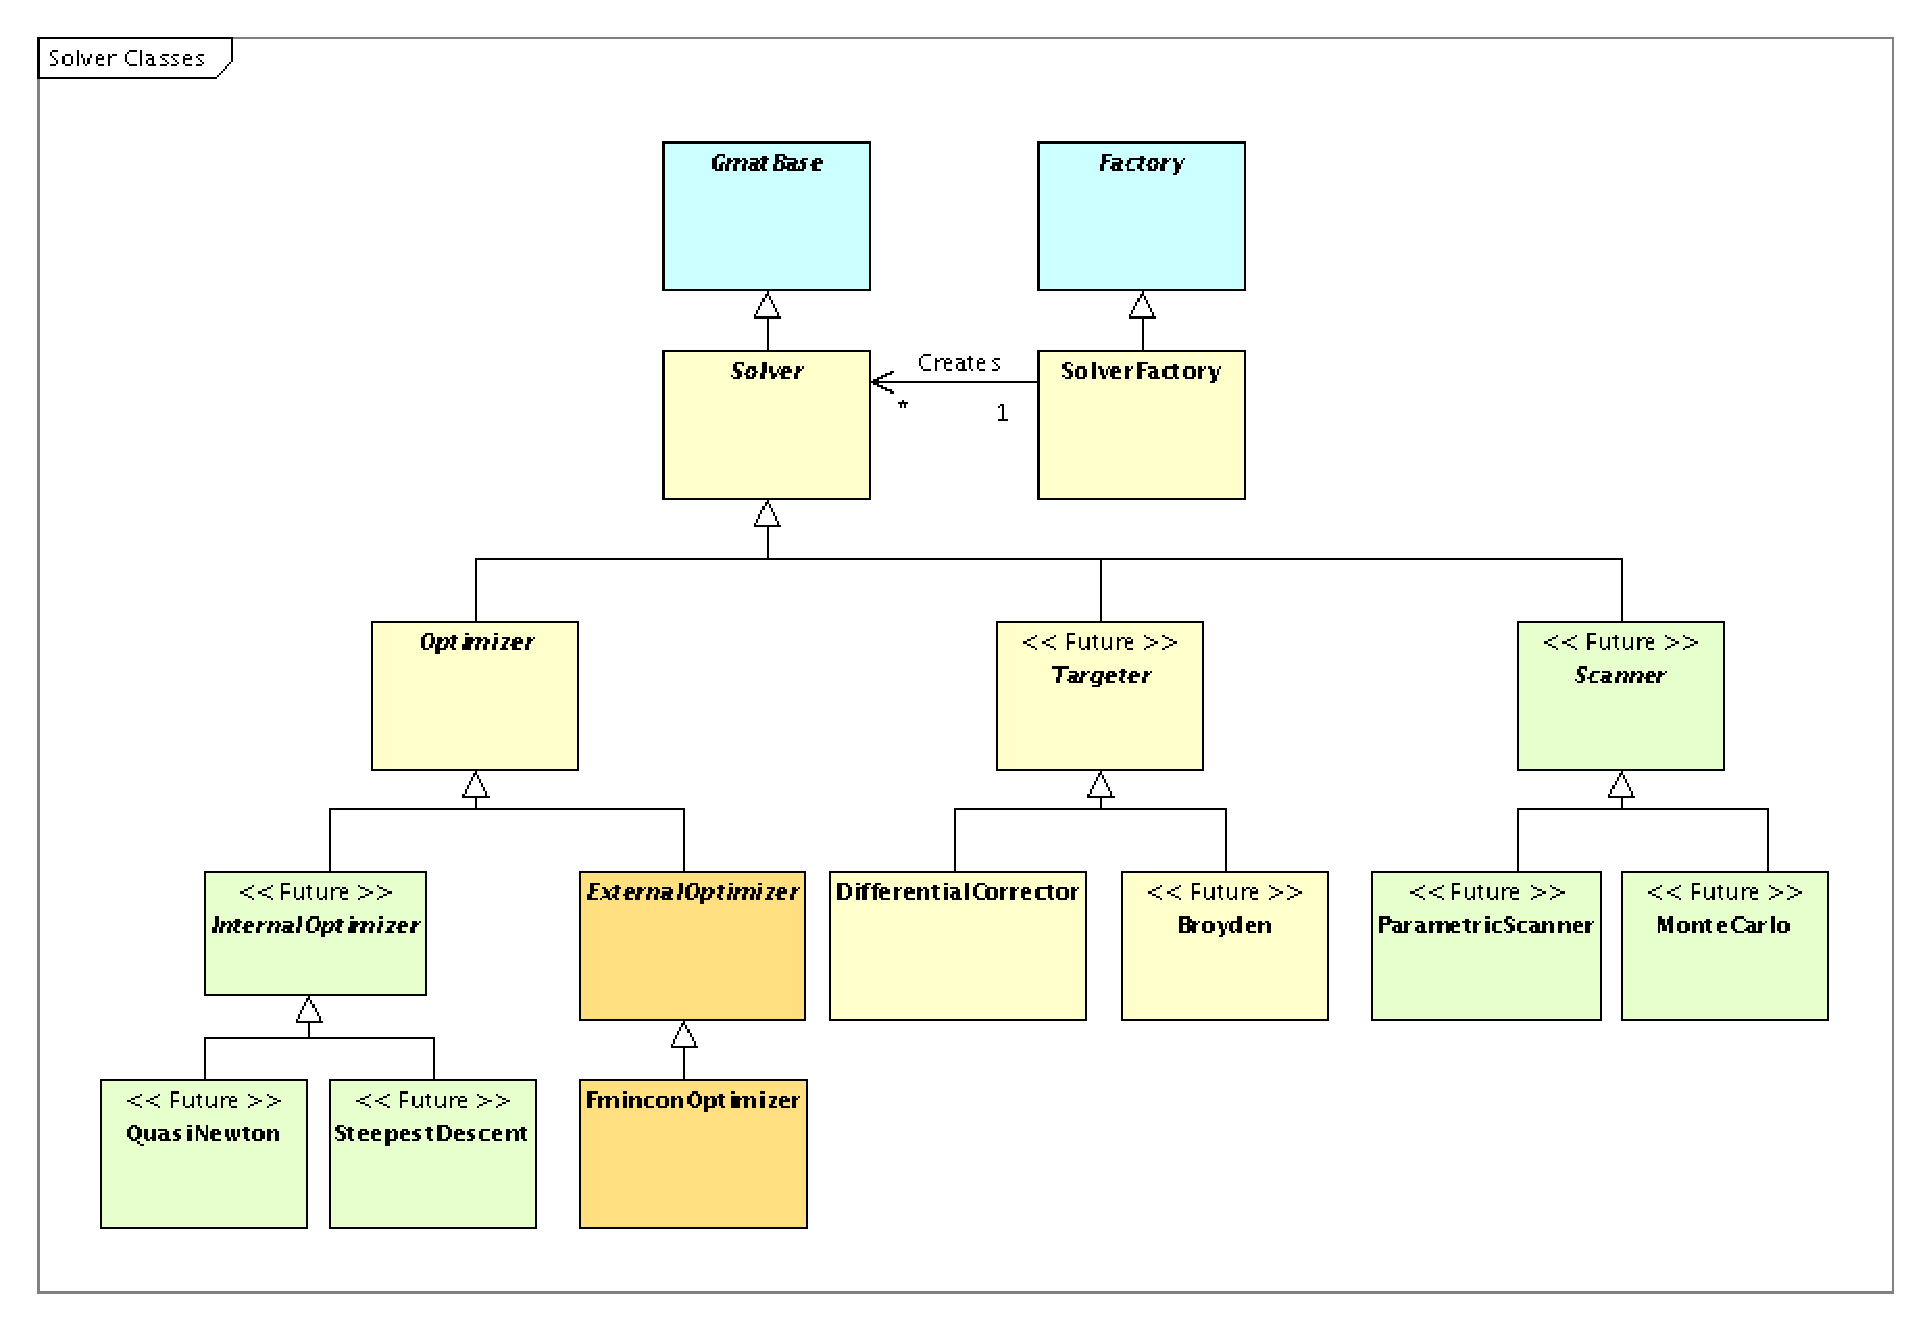
\includegraphics[scale=0.5]{Images/SolverClasses.eps}
\caption{\label{figure:SolverClasses}The Solver Subsystem}
\end{center}
\end{figure}

Figure~\ref{figure:SolverClasses}\footnote{\textbf{Note}: The current implementation of the
differential corrector does not yet conform to the class structure defined here because the
intermediate class, Targeter, is not yet implemented.} shows the class hierarchy for the GMAT
solvers, including a number of planned extensions that are not yet scheduled for implementation,
identified by the <<future>> label. The base class, Solver, contains the core elements required to
implement the solver finite state machine.  These elements are assembled differently to implement
different classes of solvers, as described in the following sections.

The Solver class hierarchy shown here identifies two scanners, two targeters (the
DifferentialCorrector and Broyden targeters), and three optimizers.  The scanners,
ParametericScanner and MonteCarlo, are planned enhancements to GMAT that are not currently scheduled
for implementation.  The DifferentialCorrector is a targeter used extensively at Goddard Space
Flight Center and other locales to find solutions to targeting goals; Broyden's method, another
targeter slated for implementation in GMAT, solves similar problems.  The SteepestDescent and
QuasiNewton optimizers are planned enhancements that will be built as native algorithms in the
GMAT code base.  The FminconOptimizer is an optimizer implemented in the MATLAB Optimization
Toolbox.  GMAT uses the MATLAB interface to communicate with this component through the
ExternalOptimizer class.

\section{The Solver Base Class}

\begin{figure}[ht]
\begin{center}
\includegraphics[scale=0.5]{Images/SolverBaseClassDetails.eps}
\caption{\label{figure:SolverBaseClass}The Solver Base Class}
\end{center}
\end{figure}

Core elements of the Solver class are shown in Figure~\ref{figure:SolverBaseClass}.  This class
contains the infrastructure required to run a solver state machine.  The class provides default
implementations for methods run at each state, and abstract interfaces for the methods used by the
GMAT Command classes.

\subsection{Solver Enumerations}

The Solver base class contains two public enumerations used evaluate the status of the solver
objects during a run and to control the style of the diagnostic reports generated by the solver.
The SolverState enumeration is used to represent the finite states in the solver's state machine.
It can be set to any of the following values:

\begin{itemize}
\item \textbf{INITIALIZING}:  The entry state for the state machine, this state is used to set
the initial data and object pointers for the state machine.
\item \textbf{NOMINAL}:  The nominal state is used to evaluate the behavior of the solver
subsequence using the current best guess at the values of the variables.
\item \textbf{PERTURBING}:  Many solver algorithms work by applying small perturbations to the
nominal values of the variables, and collecting the resulting affects on the solver subsequence.
This state is used to perform those perturbations.
\item \textbf{ITERATING}:  The Scanners perform a series of runs at calculated values of the
variables.  This state is used to iterate over those values.
\item \textbf{CALCULATING}:  The CALCULATING state is used to perform algorithm specific
calculations in preparation for the next pass through the solver subsequence.
\item \textbf{CHECKINGRUN}:  This state is used to evaluate the current results of the solver run,
and to determine if the solver algorithm has accomplished its goals.
\item \textbf{RUNEXTERNAL}: The state used to launch an external solver which controls the solution
process.
\item \textbf{FINISHED}:  This final state is used to report the results of the solver run, and to
perform any final adjustments required to use those results in the rest of the mission sequence.
\item \textbf{UNDEFINED\_STATE}:  A value used to indicate a fault, and as a special case for the
solver text file.
\end{itemize}

\noindent The states actually used by a solver are algorithm dependent; no given algorithm is likely
to use all of the states represented by this enumeration.

The ReportStyle enumeration is used to set the level of reporting performed while a solver is
executing.  This enumeration is used to represent the following styles of reporting:

\begin{itemize}
\item \textbf{NORMAL\_STYLE} The default report style, set using the string ``Normal''.
\item \textbf{CONCISE\_STYLE} A compact report style, set using the string ``Concise''.
\item \textbf{VERBOSE\_STYLE} A report style generating lots of data, useful for analyzing the
details of a run, set using the string ``Verbose''.
\item \textbf{DEBUG\_STYLE} A report style useful for debugging solver algorithms, set using the
string ``Debug''.
\end{itemize}

\noindent Each solver has a member parameter, the ``ReportStyle'', used to set the reporting style.
The ReportProgress method, described below, is used to generate the text for a report.

\subsection{Solver Members}

The Solver base class contains the following member data elements:

\subparagraph{\textit{Class Attributes}}
\begin{itemize}
\item \textbf{SolverState currentState}: The current state of the solver, one of the members of the
SolverState enumeration.
\item \textbf{std::string textFileMode}: The string representation for the output mode, set to one
of the following: ``Compact'', ``Normal'', ``Verbose'', or ``Debug''.
\item \textbf{bool showProgress}: A flag used to toggle the progress report on or off.
\item \textbf{Integer progressStyle}: An integer representation of the report style, taken from the
ReportStyle enumeration.
\item \textbf{std::string debugString}: A string used in the progress report when in Debug mode.
\item \textbf{Integer variableCount}: The number of variables used in the current problem.
\item \textbf{StringArray variableNames}: A string array containing the name of each variable.
\item \textbf{std::vector<Real> variable}: The array of current values for the variables used by the
solver.
\item \textbf{Integer iterationsTaken}: The number of iterations taken by the current run of the
solver.
\item \textbf{Integer maxIterations}: The maximum number of iterations through the subsequence
allowed for the solver.
\end{itemize}

\noindent All solvers must provide implementations of these five pure virtual methods:

\subparagraph{\textit{Abstract Methods}}
\begin{itemize}
\item \textbf{bool Initialize()}: Used to set object pointers and validate internal data
structures.  GMAT initializes all of the commands in the solver subsequence before executing this
method, so all of the variable data and result data structures have been registered when this method
is called.
\item \textbf{Integer SetSolverVariables(Real *data, const std::string \&name)}: This is the
variable registration method, used to pass in parameter data specific to variables used in the
solver algorithm.  This method is used by the Vary Command during initialization to set up the
solver variables for a run.  The return value from the method is the index in the solver array for
the variable, or -1 if the variable could not be registered.  The parameters in the method are used
to set the details for the variables:
\subitem \textit{data}: An array containing the initial value for the variable. This array may also
contain additional algorithm specific variable settings; for instance, the perturbation for the
variable, and the minimum and maximum values for the variable, and the maximum allowed step for
changes to the variable.
\subitem \textit{name}: The string name associated with the variable.
\item \textbf{Real GetSolverVariable(Integer id)}: Used to obtain the current value of a variable
from the solver.  The Vary command uses this method to refresh the current value for a variable
during a solver subsequence run.  The parameter, \textit{id}, is the index of the requested
variable in the solver's variable array.
\item \textbf{Integer SetSolverResults(Real *data, const std::string \&name, const std::string
\&type)}: This is the method used to register the values returned from the solver subsequence to
the solver.  It is used to pass in parameter data specific to the subsequence run outputs, so that
the solver has the data needed to initialize and track the results of an iteration through the
subsequence.  For targeters, the Achieve command uses this method to set up targeter goals.
Optimizers use this method to set up the connection to the objective function and constraints.
Scanners use this method to report the products of each scanning run.
\subitem \textit{data}: An array containing settings for the solver result, if applicable. An
example of the type of data in this field is the acceptable tolerance for a targeter goal.
\subitem \textit{name}: The string name associated with the solver result.
\subitem \textit{type}: The string name associated with the type of solver result.  This field
defaults to the empty string, and is only used when a solver needs to distinguish types of resultant
data.
\item \textbf{void SetResultValue(Integer id, Real value)}:  Used to report data
calculated while running the subsequence to the Solver.  Commands specific to the different
algorithms use this method to pass data into a solver; for example, for the differential corrector,
the Achieve command passes the achieved data to the solver using this method.  Optimizers use this
method to send the value of the objective function, and constraints, and, if calculated, the
gradient of the objective function and Jacobian of the constraints.  Scanners use this method to
receive the data that is being measured, so that meaningful statistics can be calculated for the
scanning run.
\end{itemize}

\noindent Each solver contains the following methods, which have default implementations:

\subparagraph{\textit{Methods}}
\begin{itemize}
\item \textbf{SolverState GetState()}:  Retrieves the current SolverState for the solver.
\item \textbf{SolverState AdvanceState()}:  Executes current state activities and then advances the
state machine to the next SolverState.
\item \textbf{void ReportProgress()}: Writes the current progress string to the GMAT message
interface, which writes the string to the log file and message window.
\item \textbf{void SetResultValue(Integer id, std::vector<Real> values)}:  Used to report multiple
data values in a vector, calculated while running the subsequence, to the solver.  Note
that this is an overloaded method; there is also an abstract SetResultValue method which sets a
single Real value.  The default implementation of this method is empty; solvers that need it should
provide an implementation tailored to their needs.
\item \textbf{void SetDebugString(std::string str)}:  Sets the string contents for the debug string.
\item \textbf{void CompleteInitialization()}:  Finalizes the initialization of the solver.  This
method is executed when the state machine is in the INITIALIZING state.
\item \textbf{void RunNominal()}:  Executes a nominal run of the solver subsequence.  This method is
executed when the state machine is in the NOMINAL state.
\item \textbf{void RunPerturbation()}: Executes a perturbation run of the solver subsequence.  This
method is executed when the state machine is in the PERTURBING state.
\item \textbf{void RunIteration()}:  Executes one run of the solver subsequence and increments the
iteration counter.  This method is executed when the state machine is in the ITERATING state.
\item \textbf{void CalculateParameters()}:  Performs algorithm specific calculations for the solver.
 This method is executed when the state machine is in the CALCULATING state.
\item \textbf{void CheckCompletion()}:  Checks to see if the solver has completed its tasks.  This
method is executed when the state machine is in the CHECKINGRUN state.
\item \textbf{void RunExternal()}:  Launches an external process that drives the solver.  This
method is executed when the state machine is in the RUNEXTERNAL state.
\item \textbf{void RunComplete()}:  Finalizes the data from the solver subsequence and sets up the
corresponding data for subsequent steps in the GMAT mission sequence.  This method is executed when
the state machine is in the FINISHED state.
\end{itemize}

\section{Scanners}

TBD -- This section will be completed when the first scanner is scheduled for implementation.

\section{Targeters}

Given a mapping from a set of variables to a set of results,

\begin{equation}\label{eq:vargoalmap}
M(x)\longrightarrow R
\end{equation}

\noindent \textit{Targeting} is the process of finding the value of a set of variables $x_G$, such
that the mapping $M(x_G)$ produces a desired set of results, $G$:

\begin{equation}\label{eq:targeting}
M(x_G) \longrightarrow G
\end{equation}

\noindent The targeting problem is a search for an exact solution.  Numerically, the targeting
problem is met when a set of variables $x_n$ is found that satisfies the conditions

\begin{equation}
M(x_n) \longrightarrow R_n \quad\quad\text{such that}\quad\vert G - R_n\vert \leq \delta
\end{equation}

\noindent where $\delta$ is the vector of tolerances for the resulting quantities.

The targeting problem is typically formulated as a series of steps proceding from an initial guess
to a solution, as outlined here:

\begin{enumerate}
   \item Generate an initial guess $x_i = x_0$
   \item\label{item:nominal} Evaluate $M(x_i) = A_i$
   \item Compare $A_i$ with the goals, $G$.  If $\vert G - A_i\vert  \leq \delta$, go to step
\ref{item:targConverged}
   \item Using the targeter algorithm, calculate new values for the variables $x_i = T(x_{i-1};
A_{i-1})$.
   \item Go to step \ref{item:nominal}
   \item\label{item:targConverged} Report the results and exit.
\end{enumerate}

\subsection{Differential Correction}

\begin{figure}[htb]
\begin{center}
\includegraphics[scale=0.5]{Images/DifferentialCorrectorStateMachine.eps}
\caption{\label{figure:DifferentialCorrectorStateMachine}State Transitions for
the Differential Corrector}
\end{center}
\end{figure}

\subsubsection{Scripting a Differential Corrector}

\begin{quote}
\VerbatimInput[numbers=left,firstnumber=1]{script/diffcorrHohmann.m}
\end{quote}


\subsection{Broyden's Method}

TBD -- This section will be completed when the Broyden's method is scheduled for implementation.

\section{Optimizers}

\textit{Optimization} is the process of taking a function $f(x)$ of a set of variables $x$, and
changing the values of those variables to move the function to a minimum.  The function $f$ is
called the objective function.  \textit{Constrained optimization} adds a set of constraints that
must simultaneously be satisfied.  More succinctly, the optimization problem can be written

\begin{equation}\label{eq:optimization}
\min_{x\in R^n} f(x) \quad \quad \text{ such that } \begin{cases}
c_i(x) = 0   \text{ and}\\
c_j(x) \geq 0
\end{cases}
\end{equation}

\noindent The constraint functions, $c$, specify additional conditions that need to be satisfied in
order for the problem to be solved.  The constraints can be broken into two categories.  Constraints
that need to be met exactly, the $c_i$ constraints in equation~\ref{eq:optimization}, are referred
to as equality constraints.  Constraints that only need to satisfy some bounding conditions,
represented here by $c_j$, are called inequality constraints.

Numerically, the optimization problem is solved when either the gradient of the objective function
falls below a specified value while the constraints are met to a given tolerance, or when the
constraints are met and the solution point $x$ is unchanging during subsequent iterations. The
optimization problem is can be formulated as a series of steps proceeding from an initial guess to a
solution, similar to a targeting problem:

\begin{enumerate}
\item Generate an initial guess $x_i = x_0$
\item Evaluate $f(x_i)$ and constraints
\item\label{item:slopeStatus} Evaluate the gradient of the objective function at $x_i$ and the
constraint Jacobians.  This step usually involves either an analytic calculation or iterating the
$f(x)$ calculation with small perturbations.
\item Check to see if $x_i$ is a local minimum or unchanging, and if the constraints are met.  If
so, go to step~\ref{item:optConverged}.
\item Use the optimizer algorithm to calculate a new search direction.
\item Step in the search direction to a minimal value in that direction.  This is the new value
for $x_i$.
\item Go to step \ref{item:slopeStatus}
\item\label{item:optConverged} Report the results and exit.
\end{enumerate}

\begin{figure}[htb]
\begin{center}
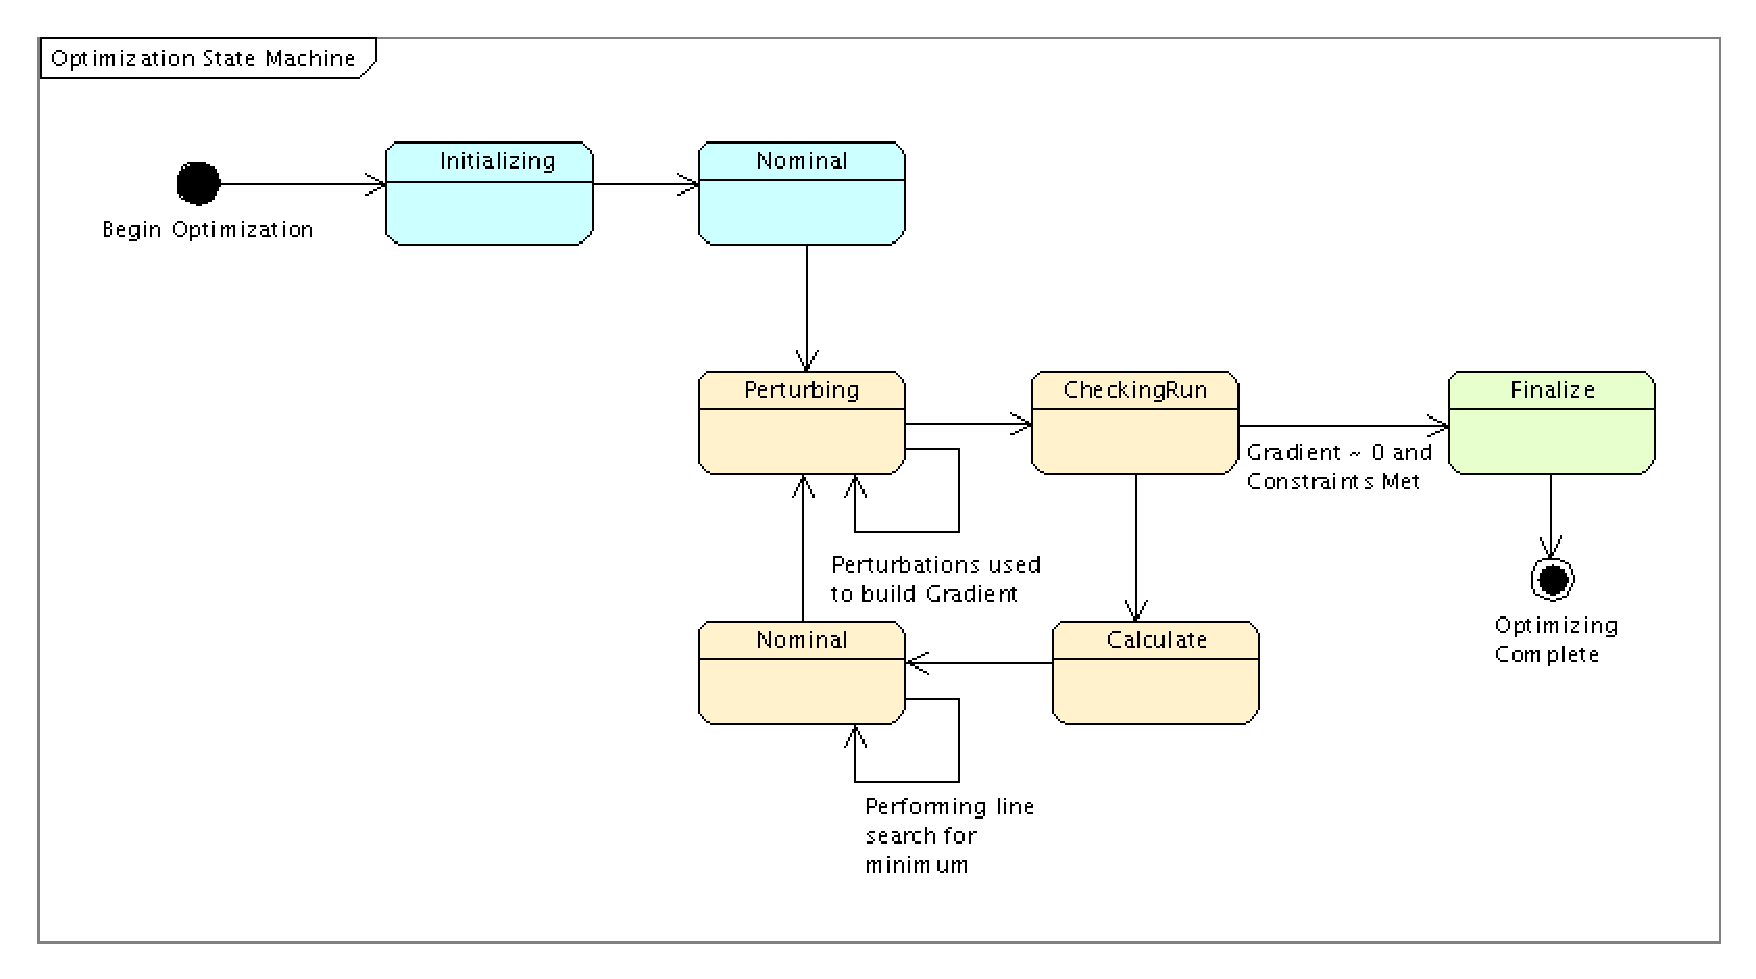
\includegraphics[scale=0.5]{Images/OptimizationStateMachine.eps}
\caption{\label{figure:OptimizationStateMachine}State Transitions for Optimization}
\end{center}
\end{figure}

\noindent Figure~\ref{figure:OptimizationStateMachine} shows the state transitions for a typical
optimization
algorithm that follows this procedure.

\subsection{The Optimizer Base Class}

\begin{figure}[htb]
\begin{center}
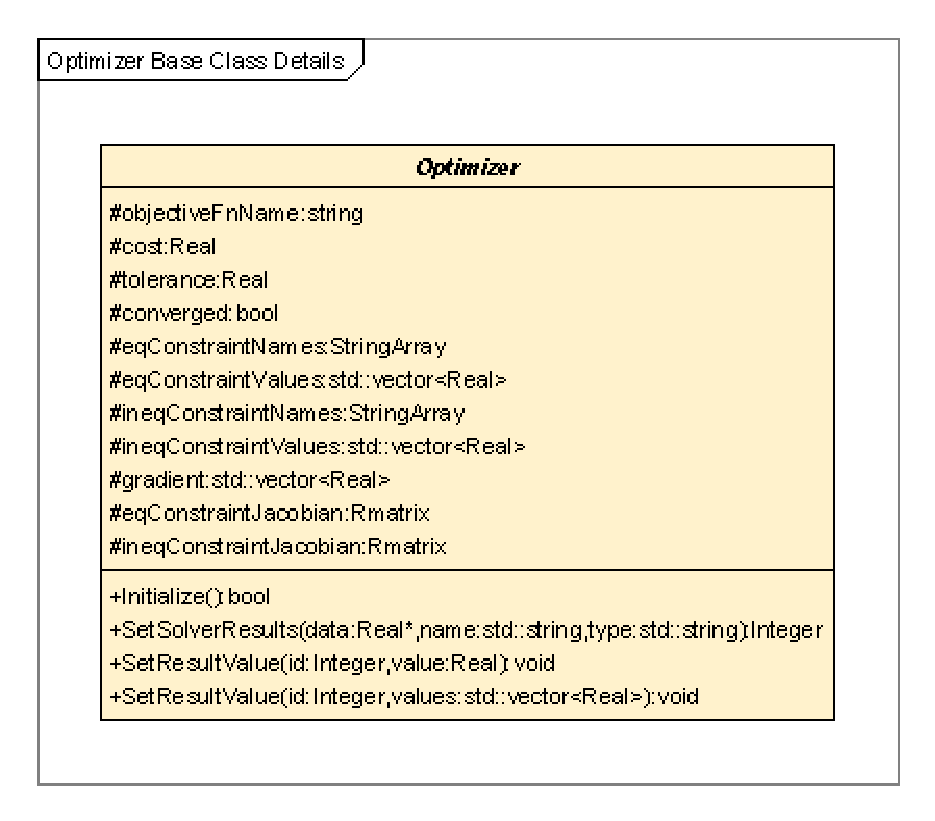
\includegraphics[scale=0.5]{Images/OptimizerBaseClassDetails.eps}
\caption{\label{figure:OptimizerBaseClass}The Optimizer Base Class}
\end{center}
\end{figure}

All optimizers require an objective function that changes based on the values of the variables in
the problem.  In addition, when analytic gradients of the objective function can be calculated, the
optimization procedure can be streamlined to incorporate these data.  Optimizers that include
constraints also need data structures to store the constraint data.  Storage support for all of
these values is built into the Optimizer base class, shown in Figure
\ref{figure:OptimizerBaseClass}.  The computation of these parameters is provided in the
optimization specific commands, described later in this chapter.  The members of this base class
serve the following purposes:

\subparagraph{\textit{Class Attributes}}
\begin{itemize}
\item \textbf{std::string objectiveFnName}: The name of the objective function data provider. This
member defaults to the string ``Objective'', but users can override that value by setting this data
member.
\item \textbf{Real cost}: The latest value obtained for the objective function.
\item \textbf{Real tolerance}: Optimizers have converged on a solution when the magnitude of the
gradient of the cost function is smaller that a user specified value.  This parameter holds that
value.  Note that GMAT can pass this parameter into external optimizers as one of the parameters
in the \textit{options} data member.
\item \textbf{bool converged}: A boolean flag used to detect when the optimizer has reached an
acceptable value for the objective function and, if applicable, the constraints.
\item \textbf{StringArray eqConstraintNames}: The names of the equality constraint variables.
\item \textbf{std::vector<Real> eqConstraintValues}: The most recent values obtained for the
equality constraints.
\item \textbf{StringArray ineqConstraintNames}: The names of the inequality constraint variables.
\item \textbf{std::vector<Real> ineqConstraintValues}: The most recent values obtained for the
inequality constraints.
\item \textbf{std::vector<Real> gradient}: <<Future>> The most recently calculated gradient of the
objective function.
\item \textbf{Rmatrix eqConstraintJacobian}: <<Future>> The most recently calculated Jacobian of the
equality constraints.
\item \textbf{Rmatrix ineqConstraintJacobian}: <<Future>> The most recently calculated Jacobian of
the inequality constraints.
\end{itemize}

\subparagraph{\textit{Methods}}  The methods shown in Figure~\ref{figure:OptimizerBaseClass} provide
implementations of the methods in the Solver base class.  These methods are described below:

\begin{itemize}
\item \textbf{bool Initialize()}: Used to set object pointers and validate internal data
structures.  GMAT initializes all of the commands in the optimizer subsequence in the
Optimize::Initialize() method, called on the command sequence during Sandbox initialization. After
performing this initialization, the Optimize command calls this method, so data structures can be
prepared for all of the variable data and result data elements registered during command subsequence
initialization.

\item \textbf{Integer SetSolverResults(Real *data, const std::string \&name, const std::string
\&type)}: Used to register parameter data needed by the optimizer to evaluate the behavior of a
subsequence run.  For optimizers, the Minimize and NonLinearConstraint commands use this method to
set up the connection to the objective function and constraints.  Future releases will implement the
Gradient, EqConstraintJacobian, and IneqConstraintJacobian commands, which will also use this
method.
\subitem \textit{data}: An array containing settings for the output parameter.
\subitem \textit{name}: The string name associated with the parameter.
\subitem \textit{type}: The string name associated with the type of resultant used in the
optimizer. Valid options are ``Objective''\footnote{If more than one command attempts to register an
objective function in the same optimizer loop, GMAT will throw an exception stating that the
optimization problem is ill defined because there is more than one objective function.},
``EqConstraint'', ``IneqConstraint'', ``ObjGradient'', ``EqConstraintJacobian'', and
``IneqConstraintJacobian''.

\item \textbf{void SetResultValue(Integer id, Real value)}:  Used to report data,
calculated while running the subsequence, to the optimizer.  The Minimize and NonLinearConstraint
commands use this method to set the current values of the objective function and constraints.

\item \textbf{void SetResultValue(Integer id, std::vector<Real> values)}:  <<Future>> Used to report
multiple data values in a vector, calculated while running the subsequence, to the optimizer.  When
implemented, the Gradient and Jacobian commands will report data to the optimizers using this
method.
\end{itemize}

\noindent Each of these methods may be overridden based on the needs of the derived optimizers.

\subsection{\label{section:InternalOptimizers}Internal GMAT optimizers}

TBD -- This section will be completed when the first internal optimizer is scheduled for
implementation.

\subsubsection{The Steepest Descent Optimizer}

TBD -- This section will be completed when the steepest descent optimizer is scheduled for
implementation.

\subsubsection{The Quasi-Newton Optimizer}

TBD -- This section will be completed when the quasi-Newton optimizer is scheduled for
implementation.

\subsection{External Optimizers}

The optimizers described in Section~\ref{section:InternalOptimizers} are coded directly into the
system.  GMAT also provides access to the MATLAB Optimization Toolbox\cite{opttools} through a set
of interfaces designed for this purpose.

\subsubsection{\label{section:ExternalOptimizationStateMachine}External Optimizer State Transitions}

\begin{figure}
\begin{center}
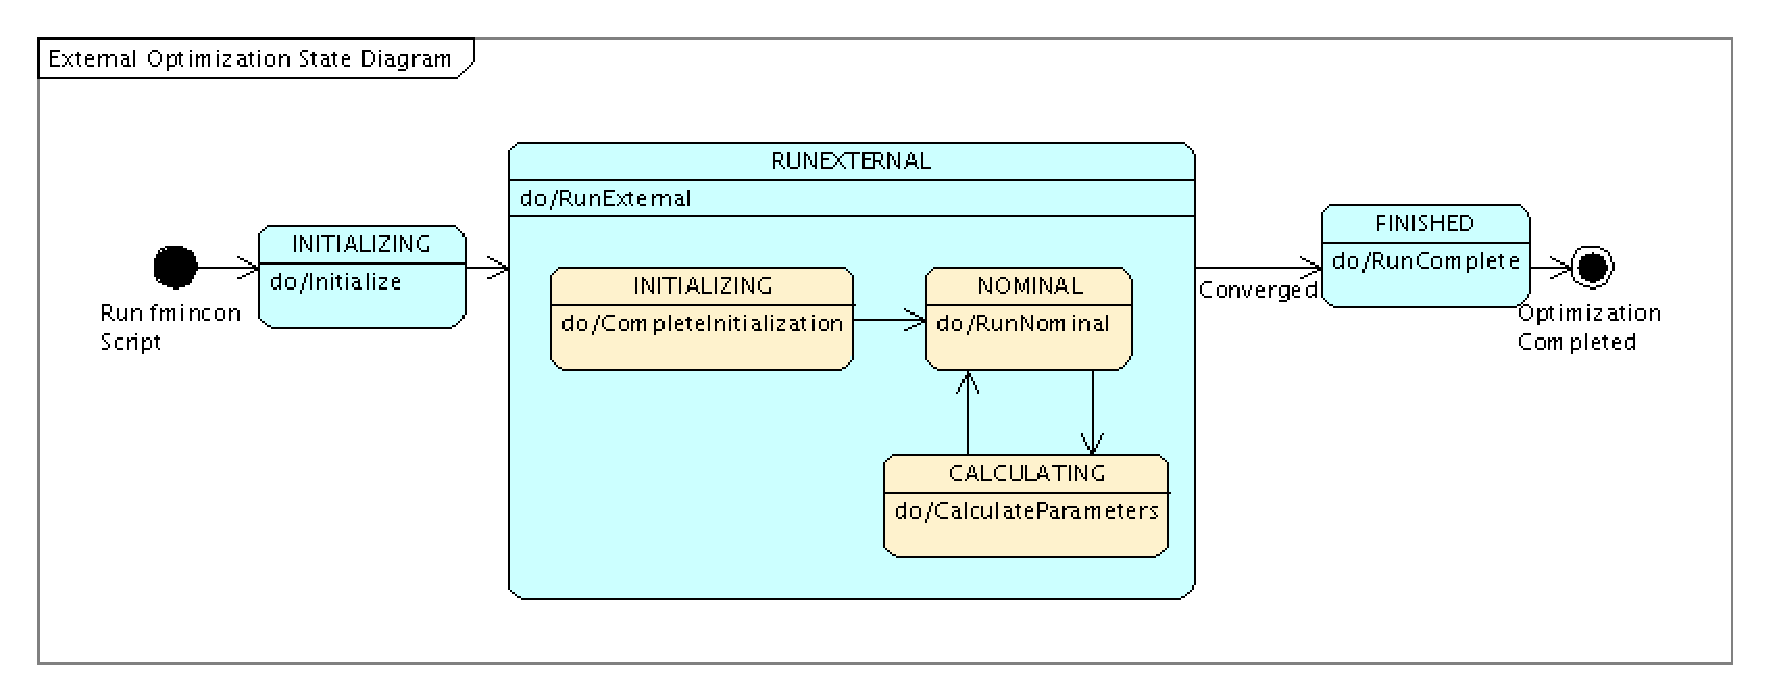
\includegraphics[scale=0.5]{Images/ExternalOptimizationStateDiagram.eps}
\caption{\label{figure:ExternalOptimizationStateDiagram}GMAT state transitions when running the
FminconOptimizer Optimizer}
\end{center}
\end{figure}

GMAT has the ability to incorporate optimizers coded outside of the system, as long at those
optimizers provide communications interfaces that can be interfaced to GMAT.  These outside
processes are called ``external optimizers.''  A typical finite state machine used to perform
optimization using an external optimizer is shown in the state transitions diagram for the fmincon
optimizer from MATLAB's Optimization Toolbox, Figure~\ref{figure:ExternalOptimizationStateDiagram}.
The state machine for fmincon will be used in what follows to provide an overvie of external
optimization; other external processes would adapt this machine to meet their needs.

The optimization process starts in an INITIALIZING state. When the AdvanceState() method is called
in this state, the object references necessary for the optimization run are set.  This step includes
passing the pointer to the Optimize command at the start of the optimization loop to the
GmatInterface that MATLAB uses to communicate with GMAT.  The Optimize command includes a method,
ExecuteCallback(), used when the fmincon optimizer needs to run the optimizer subsequence and gather
the resulting data.

Once initialization has been performed, the state transitions to the RUNEXTERNAL state. This state
calls MATLAB with the appropriate parameters needed to run the optimizer using the
FminconOptimizationDriver MATLAB function, a driver function tailored to fmincon described below.
At this point, control for the optimization process has been transferred to MATLAB.  The fmincon
optimizer makes calls back into GMAT when it needs to collect data from the optimizer subsequence.
These calls are passed to the ExecuteCallback() method registered in the initialization process,
above.  ExecuteCallback() uses the Optimize command to run the nested state transitions shown in the
figure.  The nested states start by setting up and running the mission subsequence, performed in the
NOMINAL state.  Once the subsequence has been run, the data gathered during the run are collected
and any processing needed on the GMAT side is performed.  This data collection is performed in the
CALCULATING state.  This completes the iteration of the nested state machine; the nested state is
set back to NOMINAL in preparation for the next call from MATLAB.  The collected data are passed to
MATLAB, and used by fmincon to determine the next action to be taken.  If fmincon has not yet found
an optimal solution, it calculates new values for the variables, and passes them into GMAT for
another pass through the nested state machine.  This process repeats until fmincon has found a
solution or reached another terminating condition.

Once fmincon has completed execution, it sends an integer flag to GMAT indicating how the
optimization process was terminated\footnote{See the Optimization Toolkit documentation for the
meaning of this flag's values; in general, if the flag is greater than zero, the optimization
process was successful.} and returns control to GMAT.  This return of control results in a
transition into the FINISHED state.  GMAT performs the tasks required at the end if the
optimization, and then continues running the mission sequence.  Details of all of these steps are
provided in the discussion discussion of fmincon optimization below.

\subsubsection{Class Hierarchy for the External Optimizers}

External optimizers are coded using the classes shown in
Figure~\ref{figure:OptimizationClassesExternalOptimizers}.  One set of external optimizers, the
functions in the Optimization Toolbox, is accessed using the MATLAB interface built into GMAT.
Those functions, in turn, use calls through the GmatServer code to access spacecraft specific models
in GMAT.  Future extensions to GMAT may use other interfaces for external optimizers.

\begin{figure}[htb]
\begin{center}
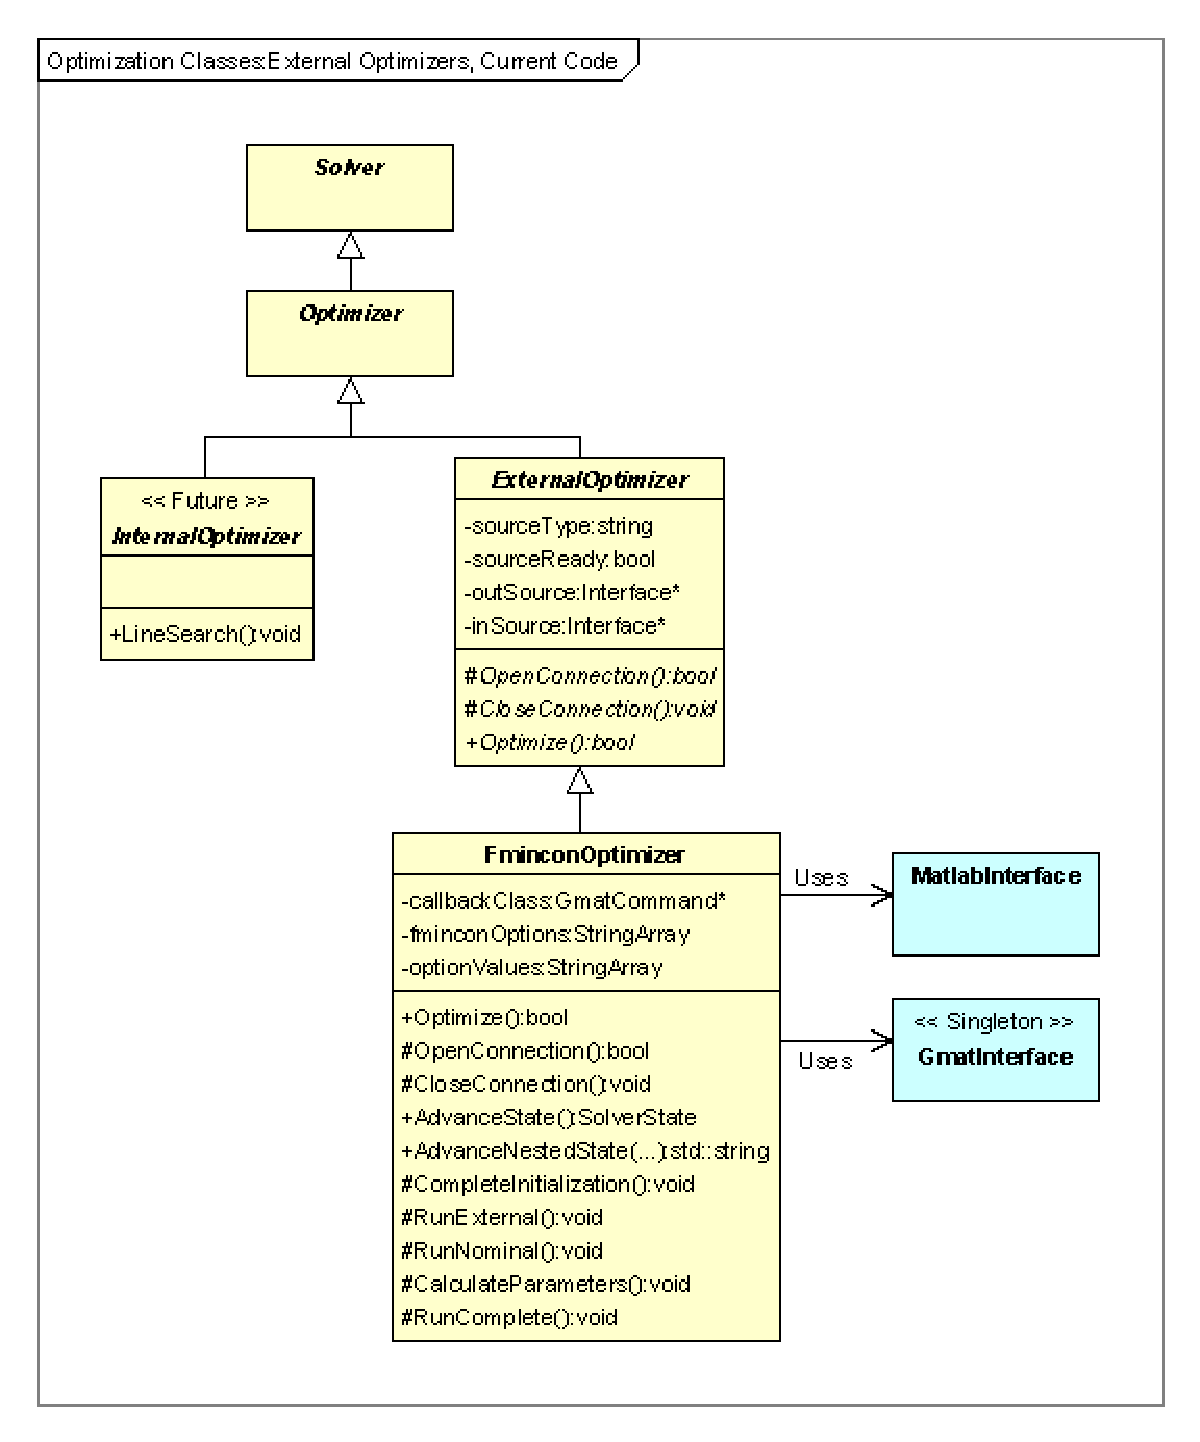
\includegraphics[scale=0.5]
{Images/OptimizationClassesExternalOptimizersCurrentCode.eps}
\caption{\label{figure:OptimizationClassesExternalOptimizers}GMAT Classes Used with External
Optimizers}
\end{center}
\end{figure}

\subsubsection{The ExternalOptimizer Class}

All external optimizers are derived from the ExternalOptimizer class.  The design illustrated in
Figure~\ref{figure:OptimizationClassesExternalOptimizers} shows this class, along with one
subclass, the FminconOptimizer, and the interfaces used to communicate with MATLAB.  When necessary,
similar interfaces will be written for communications with other external programs.  External
optimizers add the functionality needed to open the interfaces to the external programs.  Classes
derived form this class implement the state transitions functions used in the external optimization
nested state machine.  The ExternalOptimizer class elements are described here:

\subparagraph{\textit{Class Attributes}}
\begin{itemize}
\item \textbf{std::string sourceType}: String indicating the type of external interface that is
used. The only external interface supported in the current code is a MATLAB interface, so this
string is always set to ``MATLAB'' in the current GMAT code.
\item \textbf{bool sourceReady}: A flag indicating the state of the interface; this flag is set to
true if the interface was opened successfully and the supporting structures needed by the
interface were found\footnote{An example of the ``supporting structures'': if the external
interface is an FminconOptimizer, then the MATLAB system and the Optimization Toolkit must both be
available for use, and the MATLAB files that establish the calls into GMAT must also be accessible
from MATLAB.}.
\item \textbf{outSource}: A pointer to the Interface object that is used to make calls to the
external interface.
\item \textbf{inSource}: A pointer to the Interface object that is used to receive calls from the
external interface\footnote{In the current code, two pointers are necessary: one to a
MatlabInterface object, and a second to the GmatServer used for calls from MATLAB to GMAT.  Future
builds may combine these interfaces.}.
\end{itemize}

\noindent All external optimizers must provide implementations of these pure virtual methods:

\subparagraph{\textit{Abstract Methods}}
\begin{itemize}
\item \textbf{bool OpenConnection()}: The method used to open the interfaces between GMAT and the
external program.  This method, called during initialization, opens the interface and verifies that
the external program is ready to interact with GMAT.
\item \textbf{void CloseConnection()}: Closes the connections to the external program.
\item \textbf{bool Optimize()}: Calls the external optimizer, starting the optimization process.
When the process terminates, this method also terminates, returning a true value if the process
reported success and a false value if the process failed.
\end{itemize}

Note that in both of the connection configuration methods, the interface interaction preserves the
interface state as needed for other objects: for example, if the interface is already open either at
the GMAT level because of user interactions or from previous initialization, then it does not open
again; the open interface is used.  Similarly, the interface is closed only if it is not in use
elsewhere -- either globally by GMAT, or by another object that is still using the interface.

\subsubsection{The FminconOptimizer Class}

Fmincon is an implementation of sequential quadratic programming, implemented in MATLAB.  GMAT
interfaces with fmincon using a class, the FminconOptimizer class, to coordinate the calls to
MATLAB to access the optimizer.  For the purposes of this discussion, the MATLAB optimizer fmincon
will be referenced by the MATLAB function name, ``fmincon''; the GMAT class that wraps that
optimizer for use by GMAT will be referenced by the class name, ``FminconOptimizer.''

The class members for the FminconOptimizer are described here.

\subparagraph{\textit{Class Attributes}}
\begin{itemize}
\item \textbf{GmatCommand *callbackClass}: A class that implements the ExecuteCallback method used
by the external process.
\item \textbf{StringArray fminconOptions}: The table of parameters that can be set on the fmincon
optimizer.
\item \textbf{StringArray optionValues}:  The current settings for the fmincon options.
\end{itemize}

Each FminconOptimizer contains the following methods, which have default implementations:

\subparagraph{\textit{Methods}}
\begin{itemize}
\item \textbf{bool Optimize()}:  The entry point for fmincon based optimization, this method is
used to call MATLAB with the settings needed for fmincon.
\item \textbf{bool OpenConnection()}: If necessary, launches the MATLAB engine and starts the
GmatServer, and then sets the engine pointer on the FminconOptimizer.
\item \textbf{void CloseConnection()}: If appropriate, closes the MATLAB engine and/or the
GmatServer.
\item \textbf{SolverState AdvanceState()}: This method is used to run the outer state machine. It
manages 3 states: the INITIALIZING state, the RUNEXTERNAL state, and the FINISHED state.
\item \textbf{std::string AdvanceNestedState(std::vector<Real> vars)}: This method is called by the
Optimize command to run the nested state machine, and managed the transitions between the NOMINAL
and CALCULATING states.  The input parameter here is a vector of the variable values used for the
nested state machine run.  The return value for this method is the resultant data from the nested
run, serialized for transport to the external process.
\item \textbf{void CompleteInitialization()}:  The method run in INITIALIZING state, which sets the
callback class pointer for the GmatInterface and prepares the GMAT side of the system for
optimization.
\item \textbf{void RunExternal()}: The method run in the RUNEXTERNAL state which builds the data
stores needed for the optimization loop, and then calls Optimize to hand program control to MATLAB.
\item \textbf{void RunNominal()}:  The method that sets up the data structures for a run of the
optimizer subsequence.  The Optimize command uses AdvanceState to run this method immediately before
running the optimization subsequence.
\item \textbf{void CalculateParameters()}:  The method that gathers the resultant data from the
subsequence run and massages it into form for transport to MATLAB.
\item \textbf{void RunComplete()}:  The method that finalizes the optimization, writing resultant
data to the solver log file and releasing any temporary data structures that were used in the
optimization process.
\end{itemize}

\subsubsection{Interface Classes: Details for the FminconOptimizer}

\begin{figure}[htb]
\begin{center}
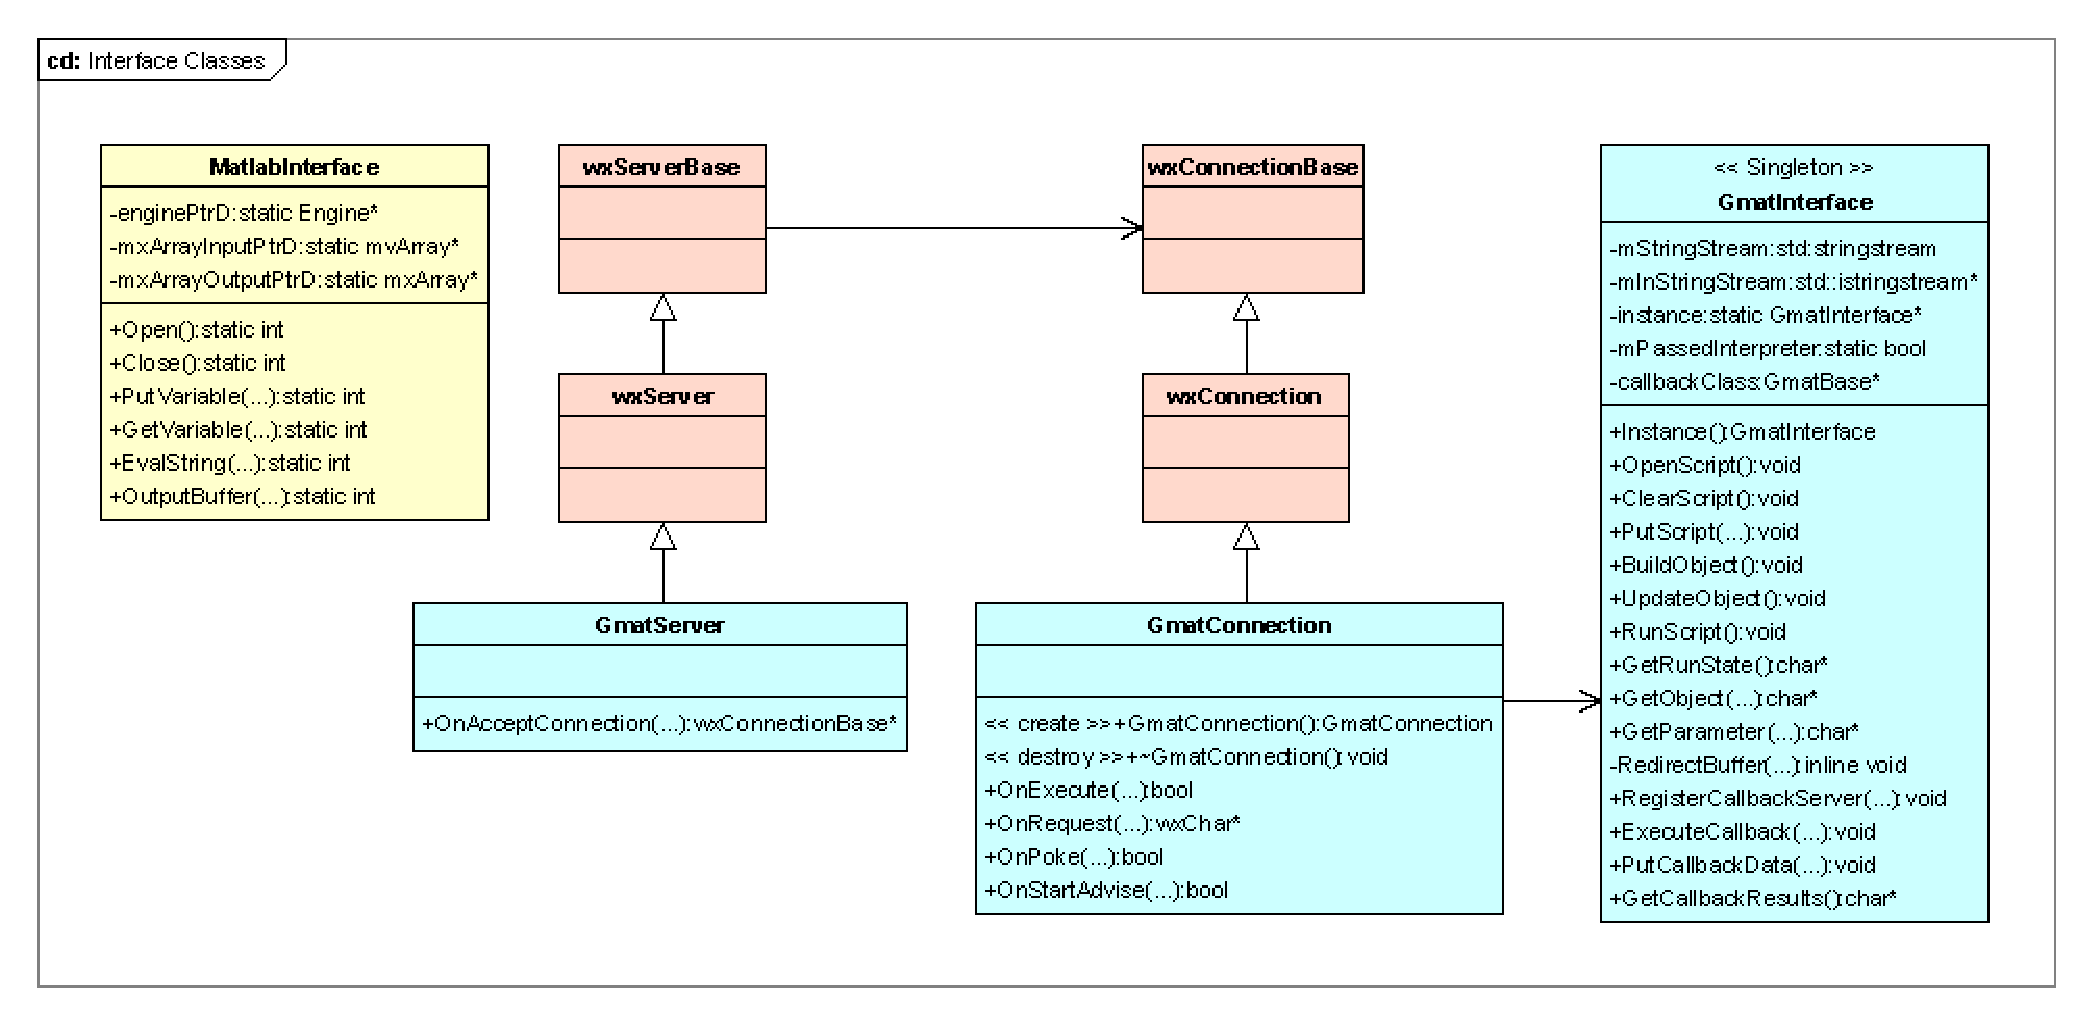
\includegraphics[scale=0.45]{Images/InterfaceClasses.eps}
\caption{\label{figure:InterfaceClasses}Interface Classes used by the FminconOptimizer}
\end{center}
\end{figure}

The current implementation of interfaces in GMAT used to communicate with MATLAB are shown in
Figure~\ref{figure:InterfaceClasses}\footnote{There are currently two separate MATLAB interfaces,
and both are used for this work.  The interface from MATLAB to GMAT uses code from the wxWidgets
library.  Because of this implementation, external optimizers running in MATLAB cannot be used with
the command line versions of GMAT.}.  Details of this implementation are provided in
Chapter~\ref{chapter:ExternalInterfaces}.  These paragraphs point out the pertinent features used
when running an external optimizer.

The Optimize command, described later, is used to control the state transitions used when running
the state machine.  This command is used to advance the state machine by calling the AdvanceState
method on the optimizer.  External optimizers use a state, the RUNEXTERNAL state, to pass control
from GMAT to the external process.  The Optimize command implements a method named ExecuteCallback
which provides the entry point from the external process back into the GMAT system so that
spacecraft modeling commands can be executed buy the external process.  The GmatInterface contains
members designed to manage this callback process.  These members, a pointer and several methods, are
described here\footnote{Note that this is not the full description of the GmatInterface class. That
description is in Chapter~\ref{chapter:ExternalInterfaces}.}:

\subparagraph{\textit{Class Attributes}}
\begin{itemize}
\item \textbf{GmatCommand *callbackClass}: A class that implements the ExecuteCallback method used
by the external process.
\end{itemize}

\subparagraph{\textit{Methods}}
\begin{itemize}
\item \textbf{void RegisterCallbackServer(GmatCommand *cbClass)}: Method used to identify the
command that implements ExecuteCallback.
\item \textbf{void ExecuteCallback()}: The method called from the GMAT server to run the callback
method.
\item \textbf{void PutCallbackData(std::string data)}: Method used to set the input data for the
callback function.  For optimization, this method is called to pass in the variable data.
\item \textbf{char* GetCallbackResults()}:  Method used to retrieve the results of the callback.
For optimization, this method retrieves the value of the objective function and constraints, and
other optional data when it becomes available.
\end{itemize}

The entry point to the optimization process is the Optimize command, described below.  When this
command is executed, the FminconOptimizer refreshes the data needed for optimization, and passes
that data across the interface to MATLAB.  These data are stored in the FminconOptimizer's

\begin{table}[tb]
\caption{\label{table:fminconOptions}Options for the FminconOptimizer Solver}
\begin{tabular}{|>{\raggedright\hspace{0pt}}p{1.2in}%
                |>{\raggedright\hspace{0pt}}p{0.6in}%
                |>{\raggedright\hspace{0pt}}p{1.3in}%
                |>{\raggedright\hspace{0pt}}p{2.5in}|}
\hline
\textbf{Option} & \textbf{Type} & \textbf{Values} & \textbf{Description}
\tabularnewline
\hline \hline
  DiffMaxChange & Real & value > 0.0 & Maximum allowed change in the variables.
\tabularnewline \hline
  DiffMinChange & Real & 0.0 < value <= DiffMaxChange & Minimum allowed change in the variables.
\tabularnewline \hline
  MaxFunEvals & Integer & value > 0 & Maximum number of function evaluations before terminating.
\tabularnewline \hline
  MaxIter & Integer & value > 0 &
\tabularnewline \hline
  TolX & Real & value > 0.0 & Variable change tolerance required to declare convergence.
\tabularnewline \hline
  TolFun & Real & value > 0.0 & Gradient tolerance required to declare convergence.
\tabularnewline \hline
  DerivativeCheck & String & On, Off & Toggle for fmincon derivative checking.
\tabularnewline \hline
  Diagnostics & String & On, Off & Toggle used to turn dignostics on for fmincon.
\tabularnewline \hline
  Display & String & Iter, Off, Notify, Final & Level of output generated from fmincon.
\tabularnewline \hline
  GradObj & String & On, Off & Toggle to turn on gradients calculated in GMAT.
\tabularnewline \hline
  GradConstr & String & On, Off & ???
\tabularnewline \hline
\end{tabular}
\end{table}

There are many different parameter settings available for MATLAB's fmincon optimizer.
Table~\ref{table:fminconOptions} shows the fmincon options supported by GMAT. The option table is
contained in the fminconOptions StringArray.  Settings for these options are collected in the
optionValues member and passed from GMAT into MATLAB when the optimization loop starts execution.

\subsubsection{Control Flow in the FminconOptimizer}

Figures~\ref{figure:ExternalOptimizationCallSequenceInit}
through~\ref{figure:ExternalOptimizationCallSequenceNestedState} show the sequence of method calls
made on the GMAT objects to run the MATLAB based fmincon optimizer.  The Optimization Toolbox
contains several other optimization functions that may be incorporated into future versions of GMAT
if the need arises; they will use a similar control flow when implemented.

\begin{subfigures}
\begin{figure}[htb]
\begin{center}
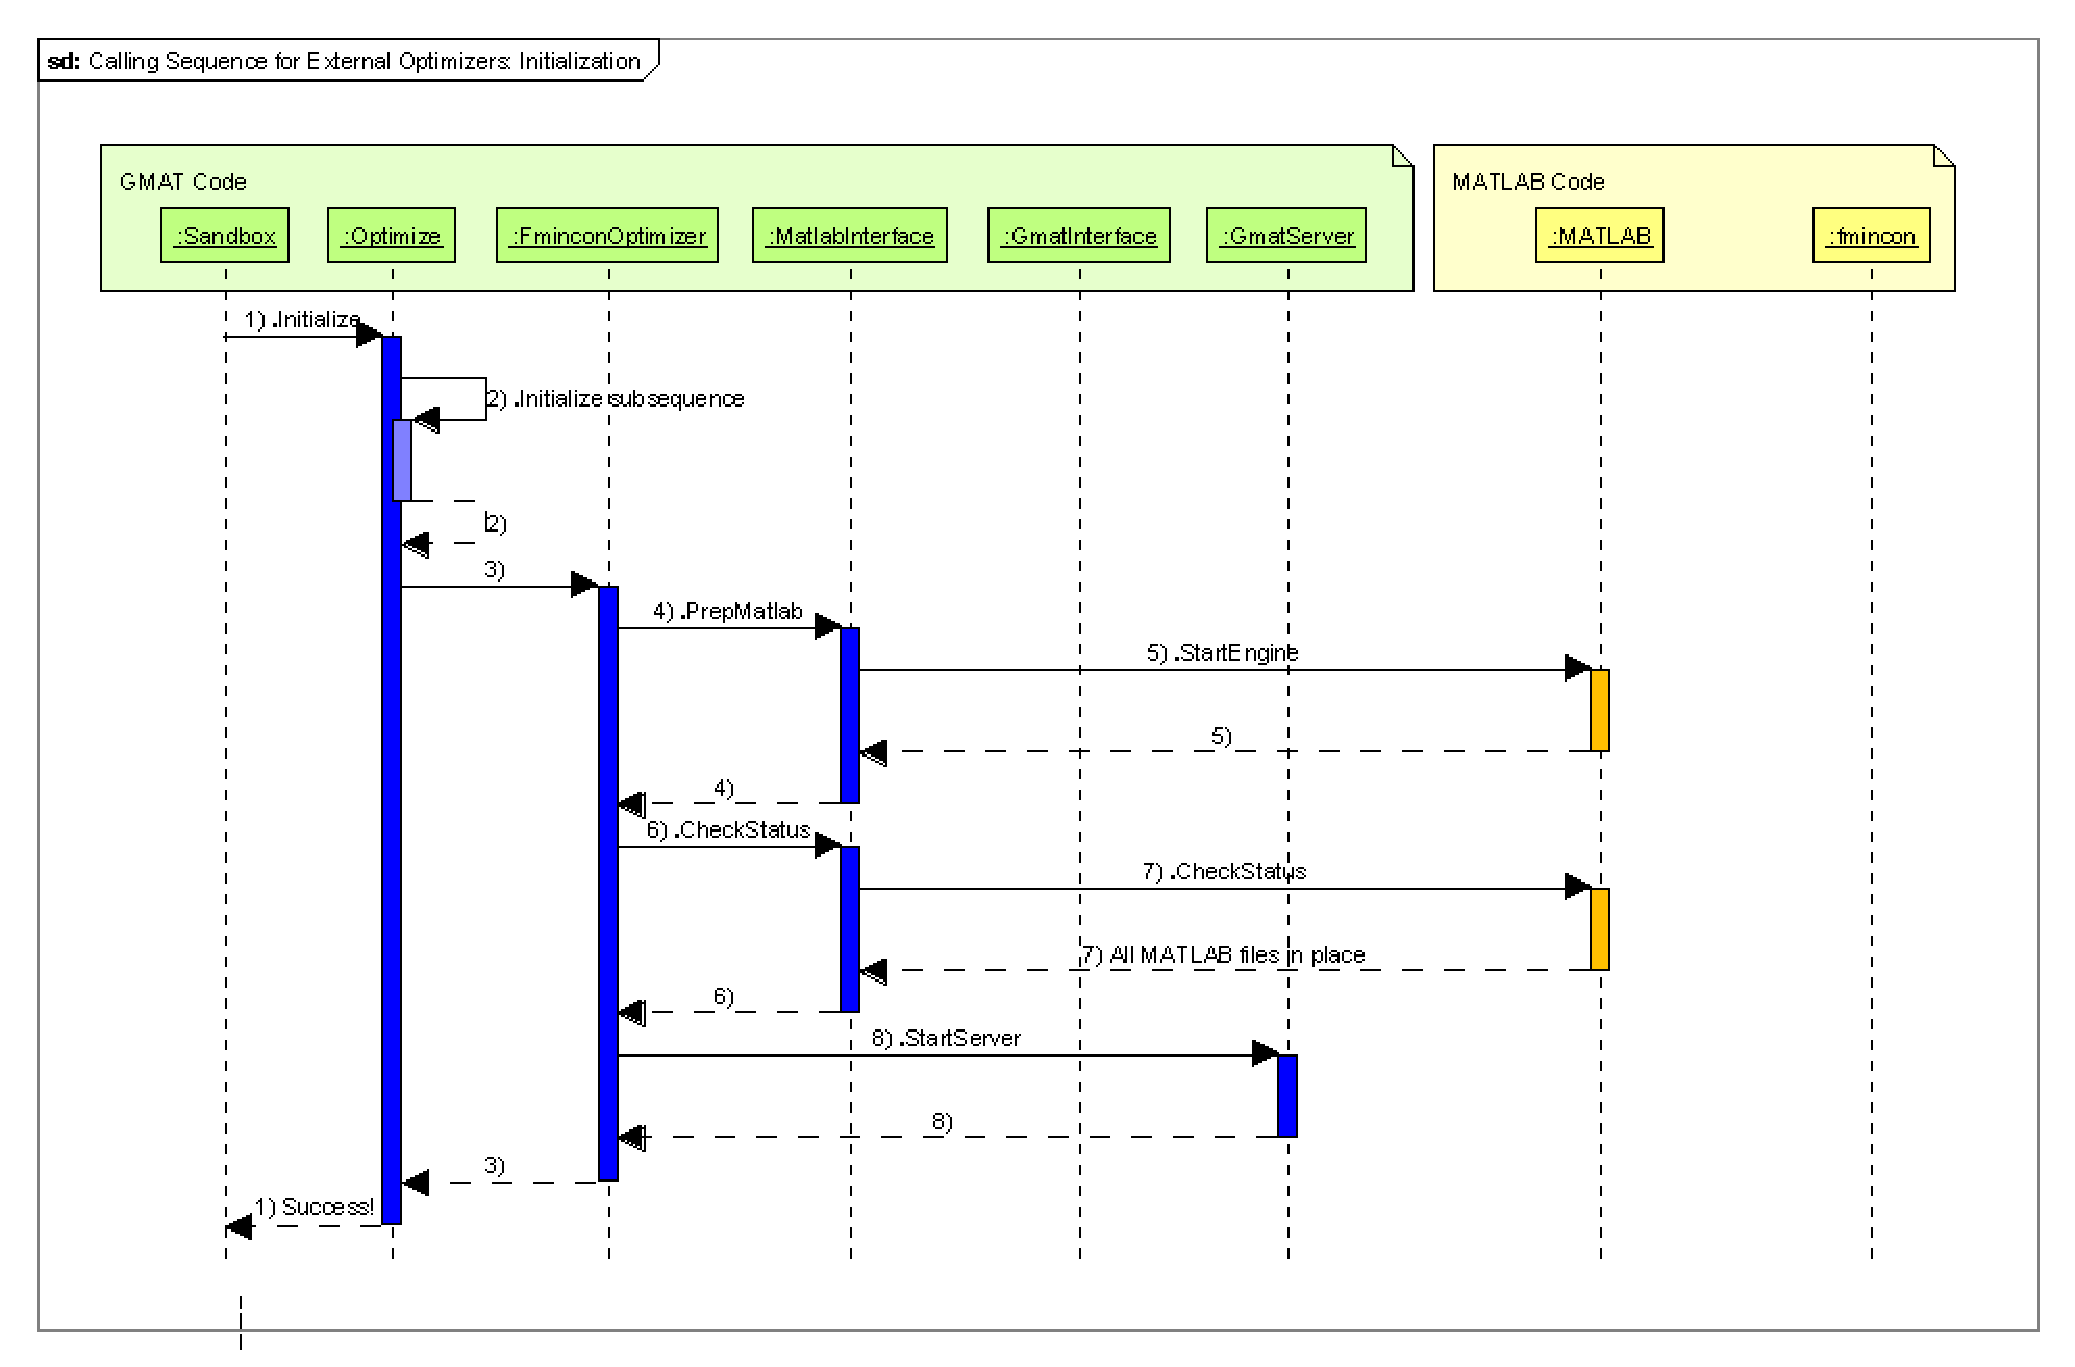
\includegraphics[scale=0.45]
{Images/CallingSequenceforExternalOptimizersInitialization.eps}
\caption{\label{figure:ExternalOptimizationCallSequenceInit}Initialization Call Sequence for
MATLAB's fmincon Optimizer}
\end{center}
\end{figure}

\begin{figure}
\begin{center}
\includegraphics[scale=0.45]
{Images/CallingSequenceforExternalOptimizersExecution.eps}
\caption{\label{figure:ExternalOptimizationCallSequenceExec}Execution Call Sequence for MATLAB's
fmincon Optimizer}
\end{center}
\end{figure}

\begin{figure}
\begin{center}
\includegraphics[scale=0.45]
{Images/CallingSequenceforExternalOptimizersNestedStateMachine.eps}
\caption{\label{figure:ExternalOptimizationCallSequenceNestedState}FminconOptimizer Nested State
Transition Details}
\end{center}
\end{figure}

\end{subfigures}

The event sequence shown in these figures consists of two pieces.  Initialization
(Figure~\ref{figure:ExternalOptimizationCallSequenceInit}) is used to set all of the object pointers
in place that are needed for the optimization, and to prepare the optimizer's internal data
structures for the optimization process.  This step includes the initialization and validation of
the interfaces used to access the external optimizer.  In the illustrated example, the input and
output interfaces GMAT uses to communicate with MATLAB are started, and the MATLAB side of the
interface validates the presence of the MATLAB scripts and functions needed to run the optimizer.
This step is performed when the GMAT Sandbox initializes the mission sequence prior to a run.

Once initialization has completed, the Sandbox starts executing the mission sequence.  The mission
sequence proceeds until the Optimize command is ready to be run.
Figure~\ref{figure:ExternalOptimizationCallSequenceExec} picks up at that point, and shows the steps
taken to perform the optimization with fmincon from within the control sequence.  These steps
include the execution of the nested state machine, described shortly.  Once the sequence shown in
this figure finishes running, the optimization process has completed, and the remainder of the
mission control sequence is run.

The details of the nested state machine run, including the execution of the optimizer subsequence,
are shown in Figure~\ref{figure:ExternalOptimizationCallSequenceNestedState}.  When
ExecuteCallback() is called on the Optimize command, the command queries the FminconOptimizer to
determine the current state of the nested state machine.  The returned state should be either
INITIALIZING or NOMINAL.

The action taken when the nested state is in the INITIALIZING state is not shown in the figure.
When that state is encountered, the Optimize command calls AdvanceNestedState on teh
FminconOptimizer and the FminconOptimizer executes its CompleteInitialization() method.
The nested state machine then transitions into the NOMINAL state.  Upon return from this process,
the Optimize command executes the StoreLoopData() method, which saves the spacecraft state data
at the start of the optimization loop.  It then proceeds to run the nested state machine.

When the nested state is in the NOMINAL state, the Optimize command calls the FminconOptimizer's
AdvanceNestedState() method, which executes the RunNominal() method to prepare the optimizer for
execution of a nominal run through the subsequence.  The state of the nested state maching changes
from NOMINAL to CALCULATING.  Upon the return from the AdvanceNestedState() method, the Optimize
command sets the GMAT objects up for a run of the optimization subsequence by executing the
ResetLoopData() method. It then begins execution of the optimization subsequence.

The execution of the optimizer subsequence depends on the order of the commands contained in the
subsequence.  All GMAT commands include a method, Execute(), that fire the command.  Like ann
GMAT command sequences and subsequences, the commands in the optimization subsequence are stored as
a linked list of GmatCommand objects. The Optimize command runs the subsequence by starting at the
begining of this linked list and firing the Execute() method on each command in the list.  The list
is navigated using the GetNext() method on the command.  The subsequence is terminated when the
GetNext() method returns a pointer to the Optimize command.

The actions shown in Figure~\ref{figure:ExternalOptimizationCallSequenceNestedState} should be
treated as a guideline for how the optimization specific commands in the subsequence interact with
the FminconOptimizer. Each time a Vary command is executed, it retrieves its variable value from
the FminconOptimizer using the GetSolverVariable() method and sets the value of the associated
variable.  The Execute() method on the Minimize command evaluates the objective function, and sends
the resulting value to the FmminconOptimizer using the SetResultValue() method.  Similarly, when a
NonLinearConstraint command is executed, the constraint is evaluated and the value is sent to the
FminconOptimizer using SetResultValue().  The order in which these actions occur is the order in
which they appear in the subsequence.

When the mission subsequence has finished execution, the Optimize command retrieves the results of
the subsequence run from the FminconOptimizer and returns these data to the GmatInterface so that
they can be passed back to MATLAB.

\subsubsection{MATLAB Support Files}

The fmincon code in MATLAB is driven from a set of three high level MATLAB function files and a
fourth lower level function.  The three high level files implement these functions:
\begin{enumerate}
\item \textbf{GmatFminconOptimizationDriver.m} manages the call into the optimizer from GMAT
\item \textbf{EvaluateGMATObjective.m} gathers data and executes the callback function into GMAT,
obtaining the data calculated in GMAT and returning the value of the objective function and
optionally its gradient
\item \textbf{EvaluateGMATConstraints.m} accesses the values for the constraints, returned in the
call to EvaluateGMATObjective.
\end{enumerate}

These three MATLAB files are listed here.  GMAT starts a fmincon run by calling the
GmatFminconOptimizationDriver function as a MATLAB function.  The actual MATLAB function syntax is
encapsulated in the FminconOptimizer; the user does not set up the function objects or the
CallFunction commands.  GmatFminconOptimizationDriver takes four inputs: a vector containing the
initial values of the variables that are being optimized, an array containing the options specified
by the user for the optimizer, as described in Table~\ref{table:fminconOptions}, and two vectors
defining the lower and upper bounds on the variables.  The function returns a vector to GMAT
containing the optimized values of the variables. The MATLAB file\footnote{This file, and all of the
other MATLAB files, are read in verbatim from the working files to ensure accuracy in the
transcription.  If you are missing any of the required files, they can be reproduced from the text
presented here.} is listed here:

\begin{quote}
\VerbatimInput{matlab/GmatFminconOptimizationDriver.m}
\end{quote}

\noindent MATLAB's fmincon optimizer uses two user supplied MATLAB functions when optimizing a
problem: one that evaluates the objective function and, optionally, its gradient, and a second that
evaluates problem constraints and the related Jacobians.  For GMAT's purposes, those two functions
are defined in the other two files listed above, EvaluateGMATObjective.m and
EvaluateGMATConstraints.m.

EvaluateGMATObjective passes the values of the variables calculated in fmincon to GMAT using the low
level CallGMATfminconSolver function, described below, and waits for GMAT to return the data
calculated off of these variables.  The variables passed to GMAT are used when running the commands
in the solver subsequence.  When GMAT receives the call from MATLAB and sets the current variable
values in the FminconOptimizer used for the mission.  Then the mission subsequence is executed one
command at a time.  Vary commands in the subsequence query the FminconOptimizer for the
corresponding variable values, and the NonLinearConstraint and Minimize, and, eventually, Gradient
and Jacobian commands set their calculated values on the FminconOptimizer as they are executed.
Once the solver subsequence finishes running, these calculated values are returned to MATLAB in the
return vectors defined for the function.  Here is the MATLAB file that implements
EvaluateGMATObjective:

\begin{quote}
\VerbatimInput{matlab/EvaluateGMATObjective.m}
\end{quote}

\noindent When control returns to MATLAB from GMAT, all of the data fmincon needs is available for
consumption.  The value of the objective function, along with its gradient if calculated, are
returned directly to fmincon.  The constraint and Jacobian data are stored in global MATLAB
variables so that they can be sent to fmincon when the optimizer requests them.  The
EvaluateGMATConstraints function provides the interface fmincon needs to access these data.  It is
shown here:

\begin{quote}
\VerbatimInput{matlab/EvaluateGMATConstraints.m}
\end{quote}

The low level callback function, CallGMATfminconSolver, uses the MATLAB server interface in GMAT to
run the solver subsequence.  This function is contained in the MATLAB file shown here:

\begin{quote}
\VerbatimInput{matlab/CallGMATfminconSolver.m}
\end{quote}

\subsubsection{Scripting the fmincon Optimizer}

A sample script for the FminconOptimizer is shown here:

\begin{quote}
\VerbatimInput[numbers=left,firstnumber=1]{script/fminconHohmann.m}
\end{quote}

\section{Command Interfaces}

The GMAT solvers are driven from a number of commands tailored to the solver algorithms.  The solver
specific commands are shown in Figure~\ref{figure:SolverCommandClasses}.  Each
category of solver is used to drive a sequence of commands that starts with the keyword associated
with the solver: ``Target'' for the targeters, ``Iterate'' for the scanners, and ``Optimize'' for
the optimizers.  The solver used for the sequence is identified on this initial line.  Each solver
sequence is terminated with a corresponding end command: ``EndTarget'' for the targeters,
``EndIterate'' for the scanners, and ``EndOptimize'' for the optimizers.  The commands enclosed
between these keywords define the variables used in the solver, the conditions that the solver is
designed to evaluate, ancillary conditions that need to be met (e.g. constraints for the
optimizers), and the sequence of events that the model runs when solving the scripted problem.  This
section describes the features of the commands that interact directly with the Solvers to solve
mission specific tasks.  The general layout and methods used by all commands are provided in
Chapter~\ref{chapter:Commands}.

\begin{figure}[htb]
\begin{center}
\includegraphics[scale=0.5]{Images/SolverCommands.eps}
\caption{\label{figure:SolverCommandClasses}Command Classes used by the Solvers}
\end{center}
\end{figure}

\subsection{\label{section:SolverCommandDescriptions}Commands Used by All Solvers}

Figure~\ref{figure:SolverCommandClasses} shows the classes used by the GMAT solvers.  Classes shown
in purple on this figure are used by targeters, in blue by scanners, and in green by optimizers.
The classes shown in yellow are base classes, and the command in orange -- the Vary command --
is used by all solvers. The solver specific commands, shown in
Figure~\ref{figure:SolverCommandsCommon}, are described in the following paragraphs.  The scripting
and options for the commands are presented first, followed by a brief description of the steps take
during initialization and execution of the commands.

\subsubsection{Solver Loop Commands}

Each solver defines a mission subsequence that starts with a command, identified by the keyword
``Target'', ``Iterate'', or ``Optimize'', followed by the name of an instantiated solver.  These
commands are collectively called the ``loop entry commands'' in the text that follows.  The commands
that are evaluated when running the solver subsequence follow this line in the order in which they
are executed.  The solver subsequence is terminated with a corresponding loop exit command, one of
``EndTarget'', ``EndIterate'', or ``EndOptimize'', selected to match the loop entry command line.
The format for a solver loop can be written

\begin{quote}
\begin{verbatim}
<LoopEntryCommand> <SolverName>
   <Solver Subsequence Commands>
<LoopExitCommand>
\end{verbatim}
\end{quote}

\begin{figure}
\begin{center}
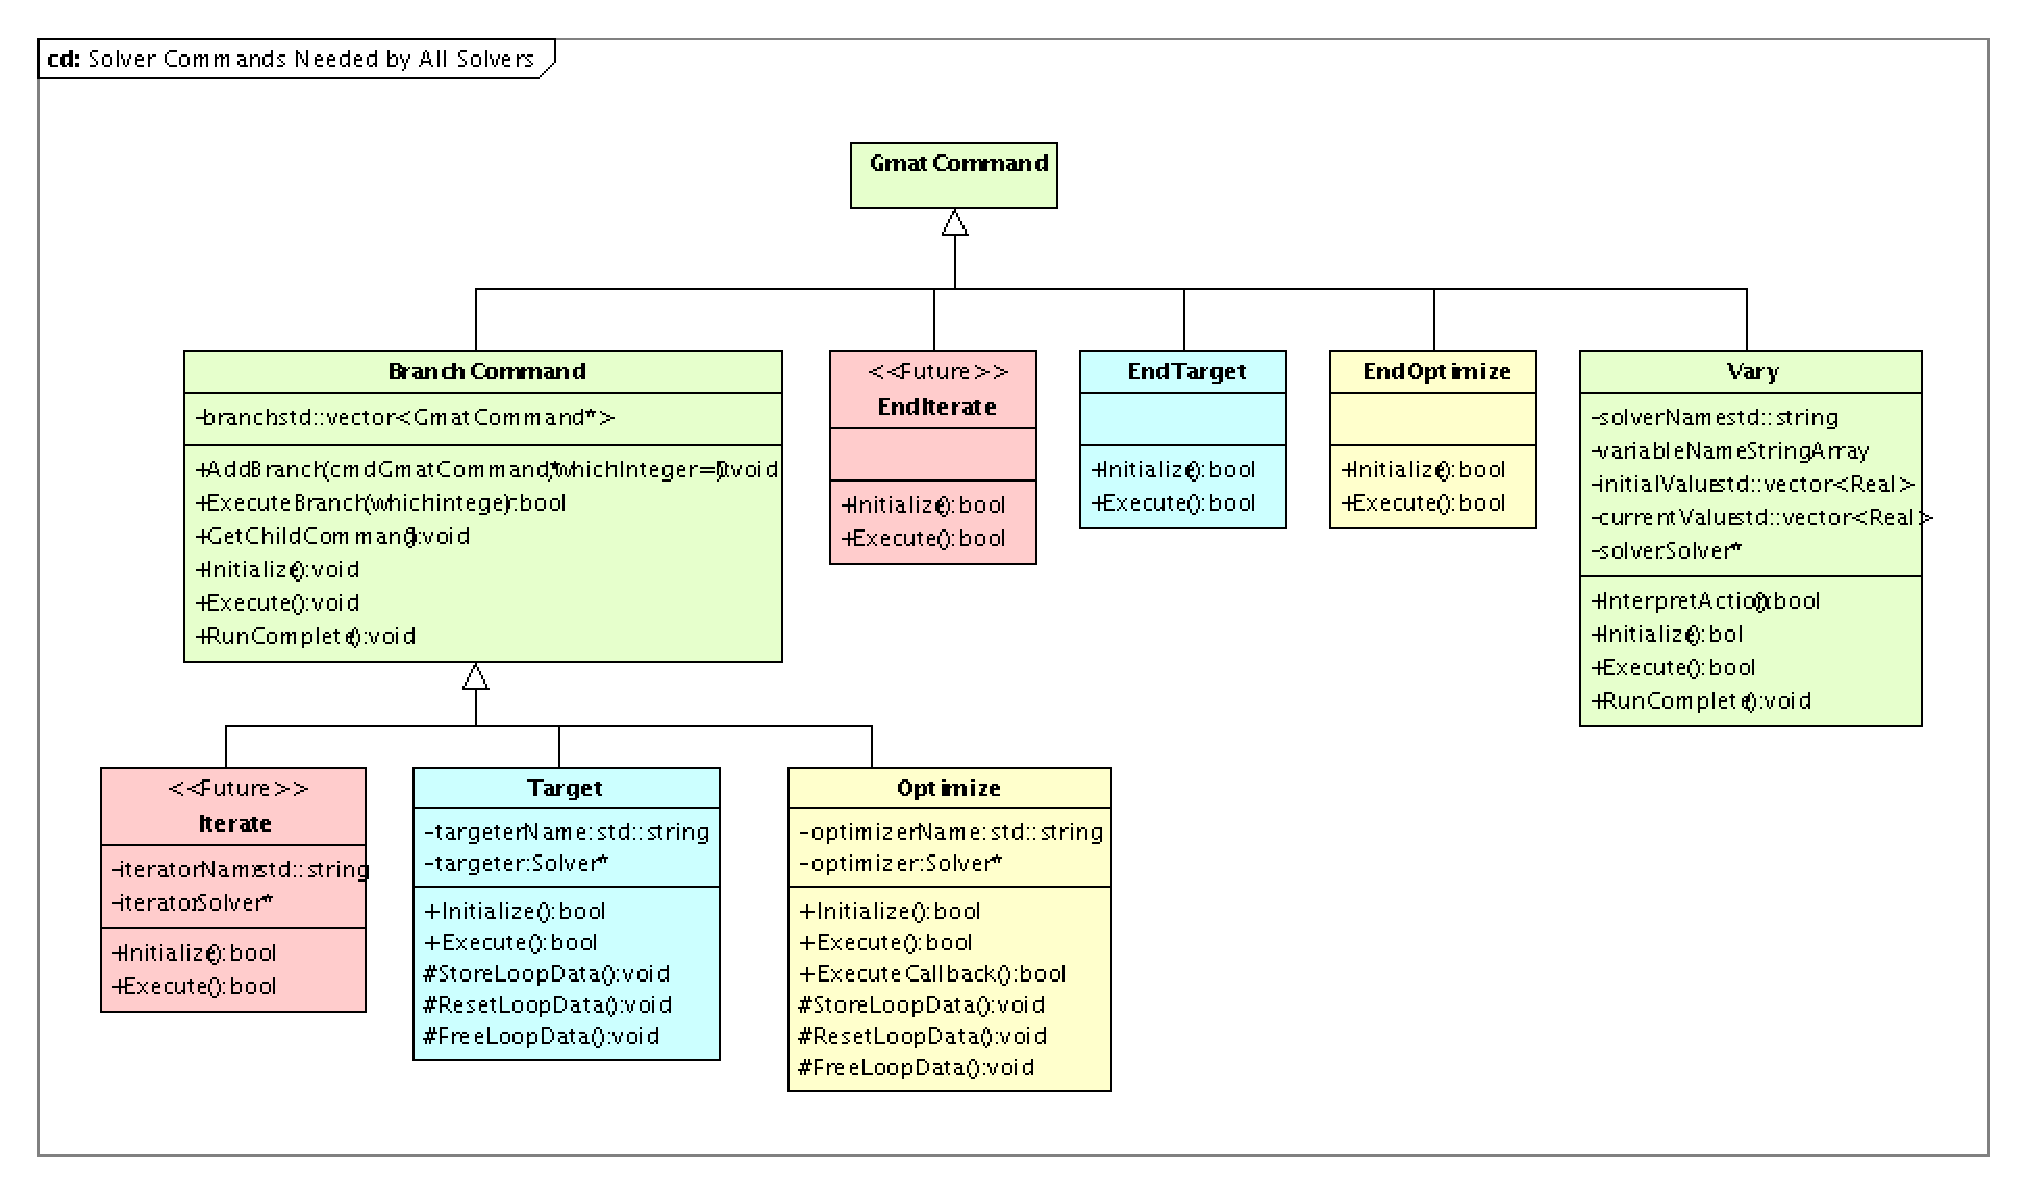
\includegraphics[scale=0.45]{Images/SolverCommandsNeededbyAllSolvers.eps}
\caption{\label{figure:SolverCommandsCommon}Command Classes Required by All Solvers}
\end{center}
\end{figure}

\noindent All solver subsequences must contain at least one \texttt{Vary} command so that the
solver has a variable to use when running its algorithm.  Targeter commands also require at least
one \texttt{Achieve} command, specifying the goal of the targeting.  Scanners require at least one
\texttt{Accumulate} command, defining the data that is collected during the iterative scan driven
by the algorithm.  Optimizers are required to define one -- and only one -- objective function,
using the \texttt{Minimize} command.

When the Solver hierarchy includes the option to drive the solution process from an external
solver, the loop entry command must also supply a method used for the external process to call back
into GMAT to run the solver subsequence.  This method, ExecuteCallback(), is currently only
supported by the optimizers.

The solver loop command members shown in the figure fill these roles:

\subparagraph{Data Elements}

\begin{itemize}
\item \textbf{std::string iteratorName, targeterName, optimizerName}: The name of the solver used
for this solver loop.
\item \textbf{Solver* iterator, targeter, optimizer}: The Solver used for this solver loop.
\end{itemize}

\subparagraph{Methods}

\begin{itemize}
\item \textbf{bool Initialize()}: Sets member pointers, initializes the solver subsequence, and then
initalizes the Solver.
\item \textbf{bool Execute()}: Runs the Solver state machine, and executes the solver subsequence
when the state machine requires it.
\item \textbf{bool ExecuteCallback()}: For external solvers\footnote{Currently only applicable for
Optimizers}, this method runs the nested state machine through one iteration.
\item \textbf{void StoreLoopData()}: Constructs objects used to store the object data at the start
of a Solver subsequence, so that the data can be reset each time the subsequence is run.  These
objects are initialized to the values of the objects at the start of the execution of the Solver
loop.
\item \textbf{void ResetLoopData()}: Resets the subsequence data to their initial values prior to
the run of the solver subsequence.
\item \textbf{void FreeLoopData()}: Releases the objects constructed in the StoreLoopData() method.
This method is called after a Solver has completed its work, immediately before proceeding to the
next command in the mission sequence.
\end{itemize}

\subparagraph{Initialization}  During initialization, the loop entry commands use the Sandbox's
local object map to find the solver used in the loop.  That solver is cloned and the clone is stored
in a local variable.  The loop entry command then walks through the list of commands in its
subsequence and passes the pointer to the solver clone into each command that needs the pointer;
these commands are those shown as solver specific in Figure~\ref{figure:SolverCommandClasses}.  The
branch command Initialize() method is then called to complete initialization of the commands in the
solver subsequence.

\subparagraph{Execution}  The loop entry commands execute by performing the following series of
events:

\begin{enumerate}
\item If the ``commandExecuting'' flag is false:
\subitem Store the current states for all spacecraft and formations
\subitem Retrieve and store the entry data for the solver
\subitem Set the ``commandExecuting'' flag to true and the and ``commandComplete'' flag to false
\subitem Retrieve the current solver state
\item \label{item:solverLoopReentryPoint} If the command is currently running the solver
subsequence, take the next step in that run. This piece is required to let the user interrupt the
execution of a run; when the subsequence is running, it periodically returns control to the Sandbox
so that the user interface can be polled for a user interrupt.
\item If the subsequence was not running, perform actions that the subsequence needs based on the
current solver state.  These actions may be restoring spacecraft data to the entry data for the
solver loop, starting a run in the mission subsequence, preparing to exit the solver loop, other
algorithm specific actions, or taking no action at all.
\item Call AdvanceState() on the solver.
\item Write out solver report data.
\item Return control to the Sandbox.
\end{enumerate}

\subsubsection{Vary}

The Vary command is used by all solvers to define the variables used by the solver, along with
parameters appropriate to the variable.  A typical Vary command has the format

\begin{quote}
\begin{verbatim}
Vary <SolverName>(<variable> = <initialValue>, {<parameter overrides>})
\end{verbatim}
\end{quote}

\noindent The \texttt{<SolverName>} should be the same solver object identified when the solver loop
was opened.  The solver must be identified in each Vary command, so that nested solvers can
assign variables to the correct solver objects\footnote{A similar constraint is applied to all
solver commands; identifying the solver removes the possibility of misassigning solver data.}.

The Vary command has the following parameters that users can override:

\begin{itemize}
\item\textbf{Pert}: Defines the perturbation applied to the variable during targeting or scanning.
This parameter has no effect when using the FminconOptimizer.  (TBD: the effect for other
optimizers.)
\item\textbf{Lower} (Default: Unbounded):  The minimum allowed value for the variable.
\item\textbf{Upper} (Default: Unbounded):  The maximum allowed value for the variable.
\item\textbf{MaxStep} (Default: Unbounded):  The largest allowed singel step that can be applied to
the variable.
\item\textbf{AdditiveScaleFactor} (Default: 0.0):  The additive factor, $A$, defined in
equation~\ref{eq:solverScaleFactors}.
\item\textbf{MultiplicativeScaleFactor} (Default: 1.0): The multiplicative factor, $M$, defined in
equation~\ref{eq:solverScaleFactors}.
\end{itemize}

\noindent Parameters are set by assigning values to these keywords.  For example, when setting
a perturbation on a maneuver component \texttt{Mnvr.V}, using the targeter dcTarg, the scripting is

\begin{quote}
\begin{verbatim}
Vary dcTarg(Mnvr.V = 1.5, {Pert = 0.001});
\end{verbatim}
\end{quote}

\noindent where the initial value for the velocity component of the maneuver is 1.5 km/s, and the
targeter applies a perturbation of 1 m/s (0.001 km/s) to the maneuver when running the targeting
algorithm.

The scale factor parameters are used to rescale the variables when passing them to the
solvers.  Scaling of the variables and other elements in a solver algorithm can be used to ensure
that the steps taken by a targeter or optimizer are equally sensitive to variations in all of the
parameters defining the problem, and therefore more quickly convergent.  When a variable is passed
to a solver, the actual value sent to the solver, $\hat{X_i}$, is related to the value of the
variable used in the solver subsequence, $X_i$, by the equation

\begin{equation}\label{eq:solverScaleFactors}
   \hat{X_i} = \frac{X_i + A}{M}
\end{equation}

\noindent where $A$ is the value set for the AdditiveScaleFactor, and M is the value of the
MultiplicativeScaleFactor.  This equation is inverted when the variable is set from the solver,
giving

\begin{equation}\label{eq:inverseSolverScaleFactors}
   X_i = M \hat{X_i} - A
\end{equation}

\noindent All solvers work with the scaled value of the variable data. When a variable value is
retrieved from the Solver, the Vary command applies equation~\ref{eq:inverseSolverScaleFactors} to
the retrieved value before using it in the mission subsequence.

The Vary command members shown in the figure fill these roles:

\subparagraph{Data Elements}

\begin{itemize}
\item \textbf{std::string solverName}: The name of the solver that uses this variable.
\item \textbf{Solver *solver}: A pointer to the Solver.
\item \textbf{std::string variableName}: The name of the variable fed by this command.
\item \textbf{<see text> initialValue}: The initial value for the variable.  This can be a number, a
piece of object data, a Parameter, or an array element.
\item \textbf{Real currentValue}: The current or most recent value of the variable.
\end{itemize}

\subparagraph{Methods}

\begin{itemize}
\item \textbf{bool InterpretAction()}: Parses the command string and builds the references needed
during initialization and execution.
\item \textbf{bool Initialize()}: Sets the member pointers and registers the variables with the
Solver.
\item \textbf{bool Execute()}: Queries the Solver for the current variable values, and sets these
values on the corresponding objects.
\item \textbf{bool RunComplete()}: Cleans up data structures used in the solver loop.
\end{itemize}

\subparagraph{Initialization}  At initialization, the Vary command registers its variable with the
solver by calling the SetSolverVariable() method.  The scaled initial value of the variable
(normalized using equation~\ref{eq:solverScaleFactors}), along with the associated parameters, are
all passed into the solver with this call. That method returns the solver's integer index for the
variable, which is stored in a member of the Vary command.

\subparagraph{Execution}  When the Vary command executes, it queries the solver for the current
value of the variable using the GetSolverVariable() method.  That method passes back the value of
the variable that should be used in the current run of the solver subsequence.  The value is
unnormalized using equation~\ref{eq:inverseSolverScaleFactors} and then used to set the value of the
variable for later use in the solver subsequence.

\subsection{Commands Used by Scanners}

Scanners are used to collect statistical data by iterating the scanner subsequence for a user
specified number of passes.  The data collected is identified using the Accumulate command, shown in
Figure~\ref{figure:ScannerCommands} and described here.

\begin{figure}[htb]
\begin{center}
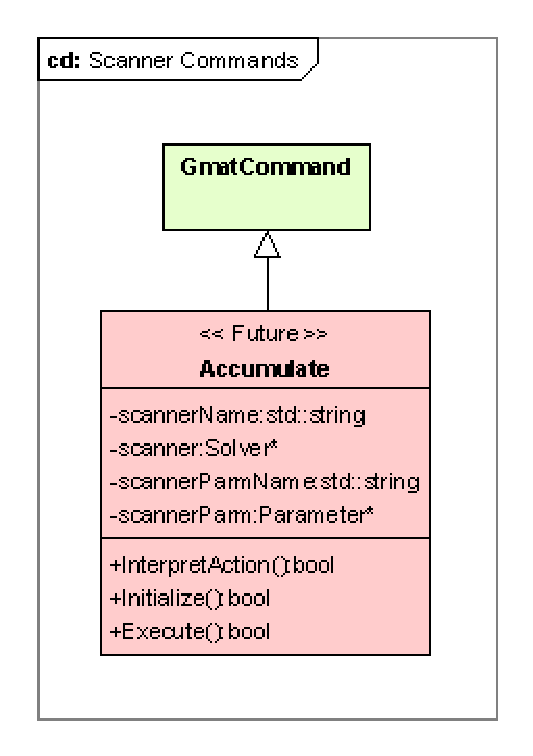
\includegraphics[scale=0.5]{Images/ScannerCommands.eps}
\caption{\label{figure:ScannerCommands}Command Classes Used by Scanners}
\end{center}
\end{figure}

TBD -- This section will be completed when the first scanner is scheduled for implementation.

\subsection{Commands Used by Targeters}

Targeters are used to change the variables so that the mission reaches some user specified set of
goals.  These goals are identified using the Achieve command, shown in
Figure~\ref{figure:TargeterCommands} and described here.

\begin{figure}[htb]
\begin{center}
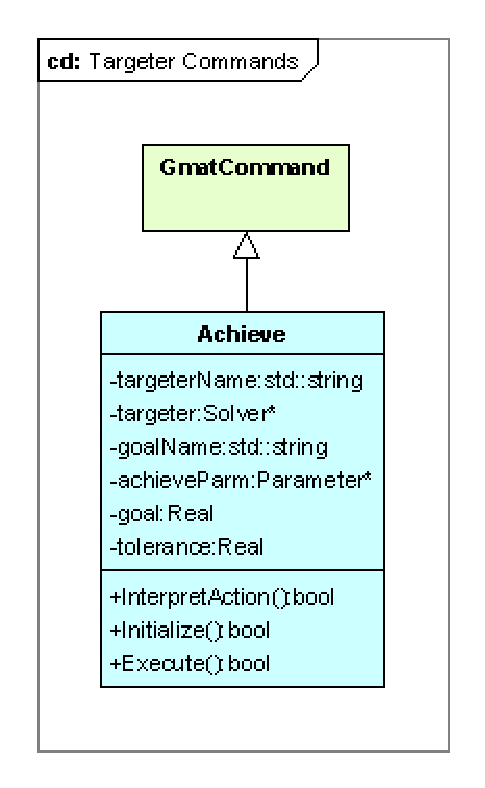
\includegraphics[scale=0.5]{Images/TargeterCommands.eps}
\caption{\label{figure:TargeterCommands}Command Classes Used by Targeters}
\end{center}
\end{figure}

\subsubsection{Achieve}

The Achieve command is used by targeters to define the goals of the targeting sequence.  Achieve
commands occur inside of a targeter subsequence.  They set the targeter goals using scripting with
the syntax

\begin{quote}
\begin{verbatim}
Achieve <TargeterName>(<goalParameter> = <goalValue>, {Tolerance = ToleranceValue})
\end{verbatim}
\end{quote}

\noindent The targeter named in the command must match the targeter named in the Target command that
starts the targeter subsequence.  The goalParameters is a GMAT Parameter that produces a Real
value. The GoalValue and the ToleranceValue each consist of  either a number, a Parameter, or an
array element, again, producing a Real number.

The Achieve command members shown in the figure fill these roles:

\subparagraph{Data Elements}

\begin{itemize}
\item \textbf{std::string targeterName}: The name of the Targeter associated with this goal.
\item \textbf{Solver *targeter}: The Targeter that is trying to meet the goal specified by this
command.
\item \textbf{std::string goalName}: The name of the parameter that is evaluated for this goal.
\item \textbf{Parameter *achieveParm}: The parameter that is evaluated for comparison with the goal.
\item \textbf{Real goal}:  The goal of the targeting run associated with the achieveParm.
\item \textbf{Real tolerance}:  The measure of how close the achieved value needs to be to the goal.
\end{itemize}

\subparagraph{Methods}

\begin{itemize}
\item \textbf{bool InterpretAction()}: Parses the command string and builds the references needed
during initialization and execution.
\item \textbf{bool Initialize()}: Sets the member pointers and registers the goals with the
Targeter.
\item \textbf{bool Execute()}: Evaluates the value of the achieveParm, and sends this value to the
Targeter.
\end{itemize}

\subparagraph{Initialization}

During Initialization, the Achieve command sets its internal member pointers and registers with the
Targeter.

\subparagraph{Execution}

When the Achieve command is executed, the parameter that calculates the current value for the
targeter goal is evaluated, and that value is sent to the Targeter.

\subsection{\label{section:OptimizationCommands}Commands Used by Optimizers}

All optimizers require exactly one Minimize command.  Optimizers may also specify other data used
in optimization; specifically, commands exist to specify nonlinear constraints, gradient data, and
Jacobian data.

\begin{figure}
\begin{center}
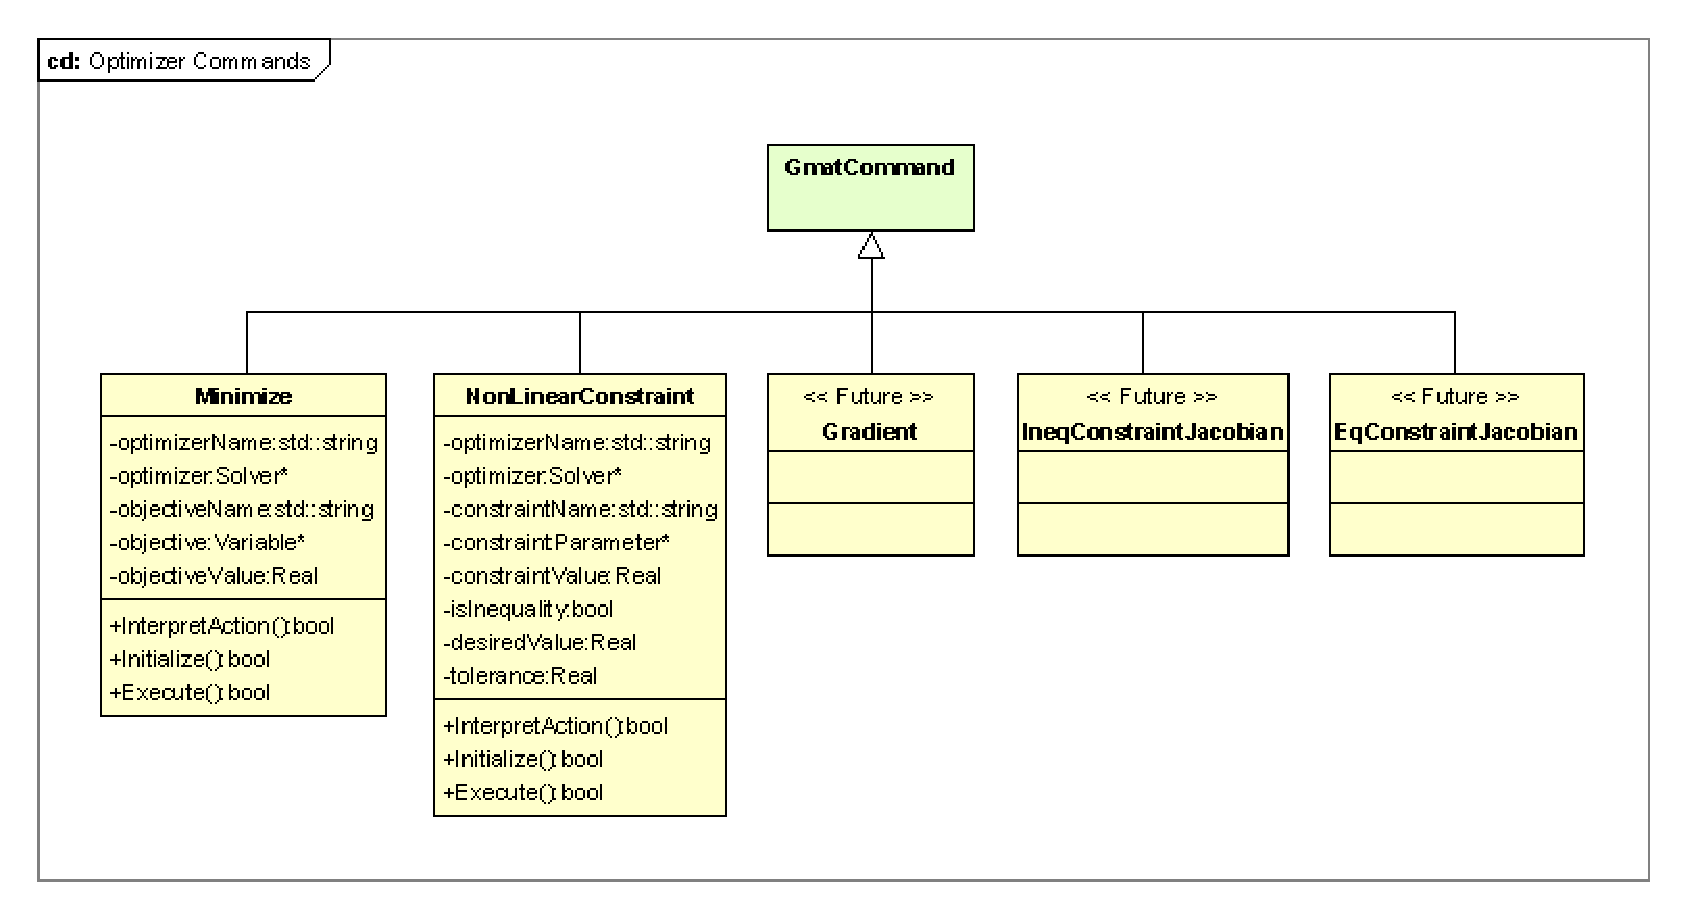
\includegraphics[scale=0.5]{Images/OptimizerCommands.eps}
\caption{\label{figure:OptimizerCommands}Command Classes Used by Optimizers}
\end{center}
\end{figure}

\subsubsection{Minimize}

The Minimize command has the syntax

\begin{quote}
\begin{verbatim}
Minimize <OptimizerName>(<ObjectiveFunction>)
\end{verbatim}
\end{quote}

\noindent As in the other solver commands, the solver identified in the command, <OptimizerName>, is
the same optimizer as was identified in the loop entry command, an Optimize command in this case.
The parameter passed inside the parentheses, identified as <ObjectiveFunction> here, returns a
scalar Real value that represents the current value of the objective function.  This function is
contained in a GMAT a Variable.

The Minimize command members shown in the figure fill these roles:

\subparagraph{Data Elements}

\begin{itemize}
\item \textbf{std::string optimizerName}: The name of the Optimizer that owns this objective.
\item \textbf{Solver *optimizer}: A pointer to the Optimizer.
\item \textbf{std::string objectiveName}: The name of the variable used to evaluate the objective
function.
\item \textbf{Variable *objective}: The variable used for the objective function.
\item \textbf{Real objectiveValue}: The current or most recent value of the objective function.
\end{itemize}

\subparagraph{Methods}

\begin{itemize}
\item \textbf{bool InterpretAction()}:  Parses the command string and builds the references needed
during initialization and execution.
\item \textbf{bool Initialize()}:   Sets the member pointers and registers the objective function
with the Optimizer.
\item \textbf{bool Execute()}:  Evaluates the value of the objective function, and sends this value
to the optimizer.
\end{itemize}

\subparagraph{Initialization}  The Optimizer used by the Minimize command is set by the Optimize
loop entry command prior to initialization of this command.  When initialization is called for the
Minimize command, the Variable providing the objective function value is found in the Sandbox's
local object map and the pointer is set accordingly.  The Minimize command then registers with the
Optimizer using the SetSolverResults method.  The Optimizer sets its member data structure
accordingly, and throws an exception if more than one objective attempts to register.

\subparagraph{Execution}  When the Minimize command is executed, the Real value of the objective
function is evaluated by calling the Variable's EvaluateReal method.  The resulting value of the
objective function is passed to the Optimizer using the SetResultValue method.

\subsubsection{NonLinearConstraint}

The NonlinearConstraint command has the syntax

\begin{quote}
\begin{verbatim}
NonlinearConstraint <OptimizerName>(<ConstraintSpecification>)
\end{verbatim}
\end{quote}

\noindent Here the OptimizerName is the name of the Optimizer identified in the Optimize loop entry
command.

The <ConstraintSpecification> has the form

\begin{quote}
\begin{verbatim}
<ConstraintParameter>  <operator>  <ConstraintValue>
\end{verbatim}
\end{quote}

\noindent <ConstraintParameter> is a Parameter, Variable, or object property.  The operator is
either an equal sign (``='') for equality constraints, or a ``<='' specification for inequality
constraints.  The constraint value is a Real number settig the target value of the constraint.

The NonlinearConstraint command members shown in the figure fill these roles:

\subparagraph{Data Elements}

\begin{itemize}
\item \textbf{std::string optimizerName}: The name of the Optimizer that owns this constraint.
\item \textbf{Solver *optimizer}: A pointer to the Optimizer.
\item \textbf{std::string constraintName}: The name of the object providing the constraint value.
\item \textbf{Parameter *constraint}: The object providing the constraint value.
\item \textbf{Real constraintValue}: The current or most recent value of the constraint.
\item \textbf{bool isInequality}: A flag indicating is the constraint is an inequality constraint.
\item \textbf{Real desiredValue}: The desired value, or right hand side, of the constraint equation.
\item \textbf{Real tolerance}: Currently unused, this is a measure of how close the calculated
value for the constraint needs to be to the actual value for equality constraints.
\end{itemize}

\subparagraph{Methods}

\begin{itemize}
\item \textbf{bool InterpretAction()}:  Parses the command string and builds the references needed
during initialization and execution.
\item \textbf{bool Initialize()}:   Sets the member pointers and registers the constraint with the
Optimizer.
\item \textbf{bool Execute()}:  Evaluates the value of the constraint, and sends this value to the
optimizer.
\end{itemize}

\subparagraph{Initialization}  The Optimizer used by the NonlinearConstraint command is set by the
Optimize loop entry command prior to initialization of this command. When initialization is called
for the NonlinearConstraint command, the object that is evaluated for the constraint is retrieved
from the Sandbox's local object map.  The constraint specification is parsed, setting the
constraint type and data in the NonlinearConstraint command.  Finally, all of the constraint
information is collected and registered with the Optimizer using the SetSolverResults method.

\subparagraph{Execution}  When the NonlinearConstraint command is executed, the Real value of the
constraint is evaluated, and the resulting value of the constraint is passed to the Optimizer using
the SetResultValue method.

\subsubsection{Gradient}

The Gradient command is used to send the gradient of the objective function to an optimizer.  This
command, a future enhancement, will be implemented when state transition matrix calculations are
incorporated into GMAT.

\subsubsection{NLIneqConstraintJacobian}

This command is used to set the Jacobian of the nonlinear inequality constraints for an optimizer.
This command, a future enhancement, will be implemented when state transition matrix calculations
are incorporated into GMAT.

\subsubsection{NLEqConstraintJacobian}

This command is used to set the Jacobian of the nonlinear equality constraints for an optimizer.
This command, a future enhancement, will be implemented when state transition matrix calculations
are incorporated into GMAT.
